\documentclass[]{usiinfthesis}

\usepackage[svgnames,table]{xcolor}
\usepackage{mdframed}
\usepackage{listings}
\usepackage{inconsolata}
\usepackage{paralist}
\usepackage{enumitem}
\usepackage{tabularx}
\usepackage{pifont}
\usepackage{multirow}
\usepackage{multicol}
\usepackage{minted}
\usepackage{todonotes}

\newcommand{\cmark}{\ding{51}}%
\newcommand{\xmark}{\ding{55}}%

\newcommand{\USI}{Universit\`a della Svizzera Italiana}


\newcommand{\hlbox}[3]{
\begin{mdframed}[backgroundcolor=#2!00]
\rightline{ \footnotesize \emph{MRQ} }
% \ 

\centering
#1
\end{mdframed}
}

\newcommand{\done}[1]{\todo[color=cyan]{\textbf{[DONE]} #1}}

\newcommand{\rquestion}[1]{\hlbox{#1}{yellow}{Research Question}}

\newcommand{\eg}{\textit{e.g.}}
\newcommand{\ie}{\textit{i.e.}}
\newcommand{\etc}{\textit{etc.}}
\newcommand{\adhoc}{\textit{ad-hoc}}
\newcommand{\perse}{\textit{per se}}
\newcommand{\circa}{\textit{circa}}

\newcommand{\phd}{Ph.D.}

\newcommand{\code}[1]{\texttt{#1}}
\newcommand{\lang}[1]{\textsc{#1}}
\newcommand{\host}[1]{\textsl{#1}}

\newcommand{\api}{API}

\newcommand{\java}{\lang{Java}}
\newcommand{\csharp}{\lang{C\#}}
\newcommand{\cc}{\lang{C}}
\newcommand{\cpp}{\lang{C++}}
\newcommand{\smalltalk}{\lang{Smalltalk}}
\newcommand{\javascript}{\lang{JavaScript}}
\newcommand{\haskell}{\lang{Haskell}}
\newcommand{\scala}{\lang{Scala}}
\newcommand{\clojure}{\lang{Clojure}}
\newcommand{\ql}{\lang{QL}}
\newcommand{\fortran}{\lang{Fortran}}
\newcommand{\cobol}{\lang{Cobol}}
\newcommand{\pascal}{\lang{Pascal}}
\newcommand{\apl}{\lang{APL}}
\newcommand{\basic}{\lang{Basic}}
\newcommand{\swift}{\lang{Swift}}
\newcommand{\php}{\lang{PHP}}
\newcommand{\racket}{\lang{Racket}}
\newcommand{\rust}{\lang{Rust}}

\newcommand{\jvm}{JVM}
\newcommand{\jvmti}{JVMTI}
\newcommand{\jni}{JNI}
\newcommand{\lilith}{Lilith}

\newcommand{\instanceof}{\code{instanceof}}
\newcommand{\throw}{\code{throw}}
\newcommand{\smu}{\code{sun.misc.Unsafe}}
\newcommand{\cce}{\code{ClassCastException}}
\newcommand{\npe}{\code{NullPointerException}}
\newcommand{\setjmp}{\code{setjmp}}
\newcommand{\longjmp}{\code{longjmp}}

\newcommand{\asm}{ASM}
\newcommand{\jnif}{JNIF}

\newcommand{\eval}{\code{eval}}

\newcommand{\github}{\host{GitHub}}
\newcommand{\gitlab}{\host{GitLab}}
\newcommand{\bitbucket}{\host{Bitbucket}}
\newcommand{\sourceforge}{\host{SourceForge}}
\newcommand{\maven}{\host{Maven}}
\newcommand{\mavencentral}{\host{Maven Central}}
\newcommand{\npm}{\host{npm}}
\newcommand{\boa}{\host{Boa}}
\newcommand{\candoia}{\host{Candoia}}
\newcommand{\lgtm}{\host{lgtm}}
\newcommand{\rascal}{\host{Rascal}}
\newcommand{\sourcegraph}{\host{sourcegraph}}

\newcommand{\unsafe}{\emph{Unsafe}}

\definecolor{lightblue}{rgb}{0,0.4,1}
\definecolor{gray}{rgb}{0.2,0.2,0.2}

\definecolor{light-gray}{rgb}{0.97,0.97,0.97}
% \definecolor{light-orange}{rgb}{1,0.6,0}
% \definecolor{light-orange}{rgb}{1,0.6,0}

\definecolor{diffstart}{named}{Grey}
\definecolor{diffincl}{named}{Green}
\definecolor{diffrem}{named}{OrangeRed}
\definecolor{hl}{named}{OrangeRed}

\setminted[java]{
	frame=lines,
	% framesep=2mm,
	baselinestretch=1.2,
	bgcolor=light-gray,
	fontsize=\footnotesize,
	% highlightcolor=light-orange,
	tabsize=4,
	linenos
}

\setminted[scala]{
	frame=lines,
	% framesep=2mm,
	baselinestretch=1.2,
	bgcolor=light-gray,
	fontsize=\footnotesize,
	% highlightcolor=light-orange,
	tabsize=4,
	linenos
}

\lstdefinestyle{java}{
	language=java,
	tabsize=4,
	basicstyle=\scriptsize\ttfamily,
	numbers=left,
	numberstyle=\tiny\color{gray},
	numbersep=4pt,
	xleftmargin=0.2cm,
	% mathescape=true,
	keywordstyle=\color{blue}\textbf,
	stringstyle=\textcolor{magenta},
	captionpos=b,
	emph={Object, String, Integer, System, ClassCastException, Foo},
	emphstyle={\color{lightblue}},
    morecomment=[f][\color{diffstart}]{@@},
    morecomment=[f][\color{diffincl}]{+\ },
	morecomment=[f][\color{diffrem}]{-\ },
}

\lstdefinestyle{ql}{
	language=sql,
	tabsize=2,
	basicstyle=\scriptsize\ttfamily,
	numbers=left,
	numberstyle=\tiny\color{gray},
	numbersep=4pt,
	xleftmargin=0.2cm,
	mathescape=true,
	keywordstyle=\color{blue}\textbf,
	stringstyle=\color{magenta},
	captionpos=b,
	showstringspaces=false,
	keywords=[2]{import, predicate, java, instanceof},
	emph={CastExpr, PrimitiveType},
	emphstyle={\color{lightblue}}
}

\lstdefinestyle{bytecode}{
	language=java,
	tabsize=4,
	basicstyle=\footnotesize\ttfamily,
	numbers=left,
	numberstyle=\tiny\color{gray},
	numbersep=4pt,
	xleftmargin=0.2cm,
	% mathescape=true,
	keywordstyle=\color{blue}\textbf,
	stringstyle=\textcolor{magenta},
	captionpos=b,
	emph={ldc,invokestatic,astore_1,aload_1,invokevirtual,checkcast},
	emphstyle={\color{lightblue}},
    morecomment=[f][\color{diffstart}]{@@},
    morecomment=[f][\color{diffincl}]{+\ },
	morecomment=[f][\color{diffrem}]{-\ },
}

\newcommand{\npattern}{31}
\newcommand{\ngroup}{10}
\newcommand{\nprim}{250}
\newcommand{\nbrokenlinks}{221}


% Change 'sl' to 'bf' for bold, or 'normalfont' for no special formatting
\captionsetup{labelfont={sl,sf}}

\title{When and How \lang{Java} Developers Give Up Static Type Safety} %compulsory
\subtitle{Subtitle: Reinventing the World} %optional 
\author{Luis Mastrangelo} %compulsory
\advisor{Prof. Matthias Hauswirth} %compulsory
\coadvisor{Prof. Nathaniel Nystrom} %optional
\Day{First} %compulsory
\Month{March} %compulsory
\Year{2019} %compulsory, put only the year
\place{Lugano} %compulsory
% Not used: Both Ph.D. Program Directors hard-coded in the class file.
\programDirector{Prof. Walter Binder \& Prof. Olaf Schenk} %compulsory

\committee{%
  \committeeMember{Prof. Antonio Carzaniga}{\USI, Switzerland}
  \committeeMember{Prof. Gabriele Bavota}{\USI, Switzerland}
  \committeeMember{Prof. Jan Vitek}{Northeastern University \& Czech Technical University}
  \committeeMember{Prof. Hridesh Rajan}{Iowa State University}
  %there can as many members as you like
} %the committee is compulsory

\dedication{To my beloved} %optional
\openepigraph{Someone said \dots}{Someone} %optional

% \makeindex %optional, also comment out \theindex at the end

\begin{document}

\maketitle %generates the titlepage, this is FIXED

\frontmatter %generates the frontmatter, this is FIXED


% DONE: Reverse the argument, we want to help, and this is how.
\begin{abstract}
The main goal of a static type system is to prevent certain kind of errors from happening at run-time.
A type system is formulated as a set of constraints that gives any expression or term in a program a well-defined type.
Yet
% DONE: "they" means all type systems, need to be more precise
% they
mainstream programming languages are endowed with type systems that
provide the means to circumvent their constraints through the \emph{unsafe intrinsics} and \emph{casting} mechanisms.

We want to understand how and when developers circumvent these constraints.
This knowledge can be:
\begin{inparaenum}[a)]
% DONE: Make a) a noun, "a ..."
% \item useful to make informed decisions for current and
% future language designers,
\item a recommendation for current and future language designers
to make informed decisions
\item a reference for tool builders, \eg{},
by providing more precise or new refactoring analyses,
\item a guide for researchers to test new language features,
or to carry out controlled programming experiments, and
\item a guide for developers for better practices.
\end{inparaenum}

We plan to empirically study how these two mechanisms
--- unsafe intrinsics and casting ---
are used by \java{} developers to circumvent the static type system.
% Our study focus on how these features are used in \lang{Java}.
% given its wide usage and relevance for both research and industry.
We have devised (%
% for the \java{}'s Unsafe \api{}
for a subset of unsafe intrinsics%
) and
% DONE: Make continuous
we are devising (for casting)
% DONE: Explain what "usage patterns" are
usage patterns,
recurrent programming idioms to solve a specific issue.
We believe that having usage patterns can help us to better categorize use cases and
thus understand how those features are used.

% These patterns can provide an insight on how the language is being used by developers in real-world applications.
\end{abstract}

% item useful to make informed decisions for current \& future language designers, not only \java{},

% Programming languages offer a wide range of features that aim to improve programmers productivity.
% However, to better drive the future evolution of any programming language,
% we believe it is AVOID:paramount to have a thorough understanding of how these features are actually being used in real codebases.

% Understanding how developers make use of language features can be helpful to a AVOID:broad audience besides language designers.
% It can aid tool builders to make more realistic assumptions;
% researchers to improve the state-of-the-art;
% and developers to implement more efficient and effective solutions by providing them best practices.

% In this proposal, we target two specific features, namely, casting and the unsafe API.
% \java{} features, namely, \emph{casting}, \emph{reflection}, \emph{exception handling} and the \emph{unsafe} \api{}.
% We give the rationale behind our decision on why we chose these features.
% We plan to devise language and API usage patterns at large-scale to properly assess this broad audience.
% We hope that having a better understanding on how these features are used, we can make informed decisions for these driving forces.


\begin{acknowledgements}

acknowledgements

\end{acknowledgements}

\tableofcontents 
\listoffigures %optional
\listoftables %optional

\mainmatter

\chapter{Introduction}

In programming language design, the main goal of a \emph{static} type system is to prevent certain kinds of errors from happening at run time.
A type system is formulated as a set of constraints that gives any expression or term in a program a well-defined type.
As~\cite{pierceTypesProgrammingLanguages2002} states:
``A type system can be regarded as calculating a kind of \emph{static} approximation to the run-time behaviors of the terms in a program.''
These constraints are enforced by the \emph{type checker} either when compiling or linking the program.
Thus, any program not satisfying the constraints stated within a type system is simply rejected by the type checker.

Besides detecting early errors,
a type checker can also be an invaluable \emph{maintenance} tool.
For instance, it can assist an IDE to perform refactoring analyses,
such as renaming a method or a field.
A static type system can be helpful to enforce disciplined programming.
When composing large-scale software,
\emph{modular languages} are built-up of types,
shown in the interfaces of modules.
Along these lines,
type systems can be useful for \emph{documentation} purposes.
Type annotations, \eg{}, in method and field declarations,
can provide useful hints to the developer.
Since type annotations are meant to be checked every time the program is compiled,
this information cannot be outdated, unlike comments in the source text.

Static type systems can aid in generating more \emph{efficient} machine code, \eg{},
choosing a different representation for integer or real values at run time.
Furthermore, in statically checked languages, \eg{}, \java{} or \rust{},
many checks are performed at compile time,
instead of being performed otherwise at run time.
Compare this to dynamically checked languages,
where all checks need to be performed at run time,
degrading performance.
Table~\ref{table:introduction:langs} shows where mainstream languages fit in the safe/unsafe and statically/dynamically checked spectrum.
``The emptiness of the bottom-right entry in the [..] table is explained by the fact that,
once facilities are in place for enforcing the safety of most operations at run time,
there is little additional cost to checking all operations.''~\citep{pierceTypesProgrammingLanguages2002}

\begin{table*}[ht]
\centering
\caption{Safe/Unsafe and Statically/Dinamically checked languages}
\label{table:introduction:langs}
\begin{tabular}{|l||l|l|}
    \hline
            & Statically checked    & Dinamically checked \\
    \hline\hline
    Safe    & \haskell{}, \ml{}, \java{}, \csharp{}, \rust{}, \etc{} & \python{}, \lisp{}, \racket{}, \etc{} \\
    Unsafe  & \cc{}, \cpp{}, \etc{} & \\
    \hline
\end{tabular}
\end{table*}


\section{Beyond Static Type Checking}

Nevertheless, often the static approximation provided by a type system is not precise enough.
Being static, the analysis done by the type checker needs to be conservative:
It is better to reject programs that are valid,
but whose validity cannot be ensured by the type checker,
rather than accept some invalid programs.
However, there are situations when the developer has more information
about the program that is too complex to explain in terms of typing constraints.
To that end, programming languages often provide \emph{mechanisms} that 
make the typing constraints less strict
to permit more programs to be valid,
at the expense of causing more errors at run time.
These mechanisms are essentially two:
\emph{Unsafe Intrinsics} and \emph{Reflective Capabilities}.

\subsection*{Unsafe Intrinsics}

Some programming languages provide \emph{unsafe intrinsics},
the ability to perform certain operations \emph{without} being checked by the compiler.
They are \emph{unsafe} because any misuse made by the programmer can compromise the entire system, \eg{},
corrupting data structures without notice, or
crashing the runtime system.
In other words,
all guarantees provided by a static type system are undermined by the inclusion of unsafe intrinsics.

Unsafe intrinsics can be seen in safe languages, \eg{},
\java{}, \csharp{}, \rust{}, or \haskell{}.
Foreign Function Interface (\emph{FFI}), \ie{}, calling native code from within a safe environment is unsafe.
This is because the runtime system cannot guarantee anything about the native code.
In addition to FFI,
some safe languages offer so-called \emph{unsafe} blocks, \ie{},
making unsafe operations within the language itself, \eg{},
\csharp{}%
\urlnote{https://docs.microsoft.com/en-us/dotnet/csharp/language-reference/language-specification/unsafe-code}
and
\rust{}.%
\urlnote{https://doc.rust-lang.org/book/second-edition/ch19-01-unsafe-rust.html}
For instance,
when using \code{unsafe} blocks in \rust{},
the developer can dereference a raw pointer,
making the application crash.

Other languages instead provide an \api{} to perform unsafe operations,
\eg{}, \haskell{}%
\urlnote{http://hackage.haskell.org/package/base-4.11.1.0/docs/System-IO-Unsafe.html}
and \java{}.
But in the case of \java{}, the \api{} to make unsafe operations,
\smu{}, is unsupported%
\urlnote{http://www.oracle.com/technetwork/java/faq-sun-packages-142232.html}
and undocumented.
For instance,
by invoking the \code{allocateInstance} on an instance of \smu{}
the developer can allocate an object without calling any constructor,
thus, violating \java{}'s type system guarantees.
\smu{} was originally intended for internal use within the \jdk{},
but as we shall see later on, it is used outside the \jdk{} as well.

\subsection*{Reflective Capabilities}

Many programming languages provide some sort of \emph{reflective capabilities},
\ie{}, they enable an executing program to examine or ``introspect'' upon itself.
Much of the \java{} Reflection \api{} resides in the \code{java.lang.reflect} package,
allowing the running program to obtain information about classes and objects.
By using reflection, it is possible to dynamically create instances of a class at run time as well, \eg{}, through the \code{Class} class.
\csharp{} provides analogous classes, \eg{}, the \code{Type} class,
to achieve the same functionality.
When reflection is used,
many checks that were done by the type checker statically (at compile time)
now need to be performed dynamically (at run time).

Programming languages with subtyping such as \java{}, \scala{} or \cpp{} provide a mechanism to \emph{view} an expression as a different type than it was defined,
a form of type introspection.
This mechanism is often called \emph{casting}.
Casting can be in two directions: \emph{upcast} and \emph{downcast}.
An upcast conversion happens when converting from a type $S$ to a type $T$, provided that $T$ is a \emph{supertype} of $S$.
An upcast does not require any explicit casting operation nor compiler check.
However, as we shall see later on,
there are situations where an upcast requires an explicit casting operation.
On the other hand,
a downcast happens when converting from a type $S$ to a type $T$,
provided that $T$ is a \emph{subtype} of $S$.

Unlike upcasts,
downcasts in a safe language require a run-time check to verify that the conversion is indeed valid.
For instance, \java{} provides the cast operator, written \code{(T) t},
while \scala{} provides the \code{asInstanceOf} method,
written \code{t.asInstanceOf[T]}.
Although \cpp{} is an unsafe language,
when used with run-time type information (RTTI),
it provides a safe cast operation, the \code{dynamic\_cast<>} operator,
written \code{dynamic\_cast<T>(t)}.
However,
\cpp{} provides more ways to perform a cast operation with different semantics that are \emph{unsafe}, \ie{},
\code{static\_cast<>},
\code{reinterpret\_cast<>},
\code{const\_cast<>}, and
\cc{}-style casts.
All mentioned cast operators in \cpp{} can perform object slicing when the type to cast to is neither a pointer nor a reference type.

This implies that downcasts provide the means to bypass the static type system.
By avoiding the type system, downcasts can pose potential threats, because it is like the developer saying to the compiler: \emph{``Trust me here, I know what I'm doing''}.
Being an escape-hatch from the static type system,
a cast is often seen as a design flaw or code smell~\citep{tufanoWhenWhyYour2015} in an object-oriented system.


\section{Research Question}

If static type systems aim to prevent certain kinds of errors from happening at run time,
yet they provide the means to loosen their typing constraints,
why exactly does one need to do so?
Are these mechanisms actually used in real-world code?
If yes, then how so?
This triggers our \textbf{main research question}:

\begin{mdframed}
\rightline{\footnotesize \emph{MRQ}}

\centering
For what purpose do developers give up static type checking?
\end{mdframed}

We have confidence that this knowledge can be:
\begin{inparaenum}[a)]
\item a reference for current and future language designers
to make informed decisions about programming languages,
\eg{}, the adoption of \emph{Variable Handles} in \java{} 9~\citep{jep193},
or the addition of \emph{Smart Casts} in \lang{Kotlin},\footnote{\url{https://kotlinlang.org/docs/reference/typecasts.html\#smart-casts}}
\item a reference for tool builders, \eg{}, by providing more precise or new refactoring analyses,
\item a guide for researchers to test new language features, \eg{}, \cite{wintherGuardedTypePromotion2011} or to carry out controlled experiments about programming, \eg{}, \cite{stuchlikStaticVsDynamic2011} and
\item a guide for developers for best or better practices.
\end{inparaenum}

To answer our question above,
we empirically studied how the two aforementioned mechanisms---unsafe intrinsics and reflective capabilities---are used by developers.
Since we seek to \emph{understand} how these mechanisms are used,
our methodology is based on qualitative analysis.
Our qualitative data to analyse is source code text
(to study unsafe intrinsics we performed a preliminary analysis on intermediate code).
In particular, in both studies we performed manual qualitative (static) analysis.
It is static because we have analysed \emph{only} the \emph{source text}
(contrast with dynamic analysis).
We performed repository mining to gather the source code text to analyse.

Since any kind of language study must be language-specific,
we focus on \java{} given its wide usage and relevance for both
research and industry.%
\footnote{\url{https://www.tiobe.com/tiobe-index/}}
Moreover, we focus on the \java{} Unsafe API to study unsafe intrinsics,
given that the \java{} Native Interface already has been studied
in~\cite{tanSafeJavaNative2006,tanEmpiricalSecurityStudy2008,kondohFindingBugsJava2008,sunNativeGuardProtectingAndroid2014,liFindingBugsExceptional2009}.
Similarly, although casting uses run-time type information like
the \java{}'s reflection \api{},
the reflection \api{} has been studied in
\cite{livshitsImprovingSoftwareSecurity2006,livshitsReflectionAnalysisJava2005,landmanChallengesStaticAnalysis2017}.

To better drive our \emph{main research question},
we propose to answer the following set of sub-questions.
To answer these research sub-questions,
we have devised \emph{usage patterns} for both the Unsafe \api{} and casting.
Usage patterns are \emph{recurrent programming idioms} used by developers to solve a specific issue.
We believe that having usage patterns can help us to better categorize use cases and
thus understand how these mechanisms are used.
These patterns can provide an insight into how the language is being used by developers in real-world applications.
Overall these sub-questions will help us to answer our MRQ:

\subsection*{Unsafe API}

\begin{enumerate}[label=$RQ/U\arabic*:$,leftmargin=3.4\parindent]
\item {\bf \urqA} \urqAdesc{}
\item {\bf \urqB} \urqBdesc{}
\end{enumerate}

The main contributions of our \unsafe{} \api{} study have been published in \conf{OOPSLA}{15}~\citep{mastrangeloUseYourOwn2015}.

\subsection*{Casting}

\begin{enumerate}[label=$RQ/C\arabic*:$,leftmargin=3.4\parindent]
\item {\bf \crqA} \crqAdesc{}
\item {\bf \crqB} \crqBdesc{}
\item {\bf \crqC} \crqCdesc{}
\end{enumerate}

The results of this study have been submitted for publication to \conf{OOPSLA}{19}.


\section{Thesis Outline}

The rest of this thesis is structured as follows.
In Chapter~\ref{cha:literature-review} we give a review of the literature in empirical studies of programming language features.
In particular, Sections~\ref{sec:literature-review:unsafe} and~\ref{sec:literature-review:casting} review the \emph{state-of-the-art} of the different aspects related to the two proposed studies.
Chapter~\ref{cha:unsafe} presents a summary of our \unsafe{} study,
while in Chapter \ref{cha:casts} we present our \emph{casting} study.
Finally, Chapter~\ref{cha:conclusions} presents the conclusions of the thesis.

The Appendix~\ref{ap:ql} contains an introduction to \ql{}%
---the language we used to approximate automatic detection of patterns---%
and reference material used in our casting study.
Appendix~\ref{ap:jnif}---although not directly related---%
describes our bytecode analysis library used in some experiments in both Chapters~\ref{cha:unsafe} and~\ref{cha:casts}.

\chapter{Literature Review}
\label{cha:literature-review}

Understanding how developers use language features
and \api{}s is a broad topic.
There is plenty of research in the computer science literature about
empirical studies of programs which involves multiple \emph{dimensions}
directly related to our plan.
Over the last decades,
researchers always have been interested in understanding what
kind of programs developers write.

The importance of conducting empirical studies of programs gave rise to the International Conference on Mining Software Repositories%
\footnote{\url{http://www.msrconf.org/}}
in 2004.

\section*{Outline}

When conducting empirical studies about programs,
multiple dimensions are involved.
The first one is \emph{What to analyse?}
Benchmarks and corpora are used as a source of programs to analyse.
Another aspect is how to select good candidate projects from a large-base software repository.
This is presented in Section~\ref{sec:literature-review:benchmarks}.
After the selection of programs to analyse is set,
comes the question \emph{how to analyse them?}
An overview of what tools are available to extract information from software repositories is given in Section~\ref{sec:literature-review:mining}.
With this infrastructure, \emph{what questions do researchers ask?}
In Section~\ref{sec:literature-review:largescale},
we give an overview of large-scale empirical studies that show what kind of questions researchers ask.
In particular, this section ends by presenting the related work more specific to the Unsafe API and Casting in Sections~\ref{sec:literature-review:unsafe} and \ref{sec:literature-review:casting} respectively.
Finally, Section~\ref{sec:literature-review:conclusions} concludes this chapter.

\section{Benchmarks and Corpora}
\label{sec:literature-review:benchmarks}

Benchmarks are crucial to properly evaluate and measure product development.
This is key for both research and industry.
One popular benchmark suite for \java{} is the DaCapo Benchmark~\citep{blackburnDaCapoBenchmarksJava2006}.
This suite has been already cited in more than thousand publications, showing how important is to have reliable benchmark suites.
The SPECjvm2008\footnote{\url{https://www.spec.org/jvm2008/}}
(Java Virtual Machine Benchmark)
and
SPECjbb2000\footnote{\url{https://www.spec.org/jbb2000/}}
(Java Business Benchmark)
are another popular \java{} benchmark suite.

Another suite has been developed by~\cite{temperoQualitasCorpusCurated2010}.
They provide the Qualitas Corpus, a corpus of curated open source systems to facilitate empirical studies on source code.
On top of the Qualitas Corpus,~\cite{dietrichXCorpusExecutableCorpus2017} provide an executable corpus of \java{} programs.
This allows any researcher to experiment with both static and dynamic analysis.

For any benchmark or corpus to be useful and reliable,
it must faithfully represent real-world code.
For instance,
DaCapo applications were selected to be diverse real applications and
ease of use, but they ``excluded GUI applications since they are difficult
to benchmark systematically.''
Along these lines, \cite{allamanisMiningSourceCode2013} go one step further and provide a large-scale (14,807) curated corpus of open source \java{} projects.

With the advent of cloud computing,
several source code management (SCM) hosting services have emerged, \eg{},
\github{}, \gitlab{}, \bitbucket{}, and \sourceforge{}.
These services allow the developer to work with different SCMs, \eg,
Git, Mercurial, Subversion to host their open source projects.
These projects are usually taken as a representation of
real-world applications.
Thus, while not curated corpora, these hosting services are
commonly used to conduct empirical studies.

Another dimension to consider when analysing large codebases, is how relevant the repositories are.
\cite{lopesDeJaVuMapCode2017} conducted a study to measure code duplication in \github{}.
They found out that much of the code there is actually duplicated.
This raises a flag when considering which projects to analyse when mining software repositories.

\cite{baxterCloneDetectionUsing1998} propose a clone detection algorithm using Abstract Syntax Trees,
while \cite{riegerVisualDetectionDuplicated} propose a visual detection for clones.
\cite{yuanCMCDCountMatrix2011,chenReplicationReproductionCode} instead propose Count Matrix-based approach to detect code clones.

\cite{nagappanDiversitySoftwareEngineering2013} have developed the Software Projects Sampling (SPS) tool.
SPS tries to find a maximal set of projects based on representativeness and diversity.
Diversity dimensions considered include total lines of code,
project age, activity, number of contributors, total code churn,
and number of commits.

\section{Tools for Mining Software Repositories}
\label{sec:literature-review:mining}

When talking about mining software repositories,
we refer to extracting any kind of information from large-scale codebase repositories. 
Usually doing so requires several engineering but challenging tasks.
The most common being downloading, storing, parsing, analysing and
properly extracting information from different kinds of artifacts.
In this scenario, there are several tools that allows a researcher or developer to query information about software repositories.

\cite{urmaProgrammingLanguageEvolution2012} evaluated seven source code
query languages:
\emph{Java Tools Language}~\citep{cohenJTLJavaTools},
\emph{SOUL}~\citep{derooverSOULToolSuite2011},
\emph{Browse-By-Query}\footnote{\url{http://browsebyquery.sourceforge.net/}},
\emph{JQuery}~\citep{volderJqueryGenericCode2006},
\emph{.QL}~\citep{moorKeynoteAddressQL2007},
\emph{Jackpot}\footnote{\url{http://wiki.netbeans.org/Jackpot}}, and
\emph{PMD}\footnote{\url{https://pmd.github.io/}}.
They have implemented, whenever possible,
four use cases using the tools mentioned above.
They concluded that only \emph{SOUL} and \emph{.QL} have the minimal features to implement all their use cases.

\cite{dyerBoaLanguageInfrastructure2013,dyerDeclarativeVisitorsEase2013} built \boa{}, both a domain-specific language and an online platform\footnote{\url{http://boa.cs.iastate.edu/}}. 
It is used to query software repositories on two popular hosting services, \github{} and \sourceforge{}.
The same authors of \boa{} conducted a study on
how new \java{} features, \eg,
\emph{Assertions},
\emph{Enhanced-For Loop},
\emph{Extends Wildcard},
were adopted by developers over time~\citep{dyerMiningBillionsAST2014}.
This study is based \sourceforge{} data.
The current problem with \sourceforge{} is that is outdated.

To this end, \cite{gousiosGHTorentDatasetTool2013} provides an offline mirror of \github{} that allows researchers to query any kind of that data.
Later on, \cite{gousiosLeanGHTorrentGitHub2014} published the dataset construction process of \github{}.

Similar to \boa{}, \lgtm{}\footnote{\url{https://lgtm.com/}} is a platform to query software projects properties.
It works by querying repositories from \github{}.
But it does not work at a large-scale, \ie{}, \lgtm{} allows the user to query just a few projects.
Unlike \boa{}, \lgtm{} is based on \ql{}---before named \emph{.QL}---,
an object-oriented domain-specific language to query recursive data structures based on Datalog~\citep{avgustinovQLObjectorientedQueries2016}.
Another static analysis framework based on Datalog is \doop{}~\citep{bravenboerStrictlyDeclarativeSpecification}.
Since \ql{} and \doop{} are based on Datalog,
both are well-suited to perform points-to analysis and data-flow analysis.
However, scaling such analysis to a large-scale study remains an open problem.

On top of \boa{},~\cite{tiwariCandoiaPlatformBuilding2017} built \candoia{}%
\footnote{\url{http://candoia.github.io/}}.
Although it is not a mining software repository \perse{},
it eases the creation of mining applications. 

Another tool to analyse large software repositories is presented in~\cite{brandauerSpencerInteractiveHeap2017}.
In this case, the analysis is dynamic, based on program traces. 
At the time of this writing, the service\footnote{\url{http://www.spencer-t.racing/datasets}} was unavailable for testing. 

\cite{bajracharyaSourcererInternetscaleSoftware2009} provide a tool to query large code bases by extracting the source code into a relational model.
Sourcegraph\footnote{\url{https://sourcegraph.com}} is a tool that allows regular expression and diff searches.
It integrates with source repositories to ease navigate software projects.

\cite{posnettTHEXMiningMetapatterns2010} have extended
\asm{}~\citep{brunetonASMCodeManipulation2002}
to detect meta-patterns, \ie{},
structural patterns of object-oriented interaction.
\cite{huDynamicAnalysisDesign2008} used both dynamic and static analysis to discover design patterns, while \cite{arcelliDesignPatternDetection2008} used only dynamic analysis.

Trying to unify analysis and transformation tools,
\cite{vinjuHowMakeBridge2006} and~\cite{klintRASCALDomainSpecific2009} built \rascal{},
a DSL that aims to bring them together by querying the AST of a program.
Spoon is a \java{} library
``to analyse, rewrite, transform, transpile \java{} source code''~\citep{pawlak:hal-01169705}.
It supports symbol resolution natively and match code elements using Spoon patterns.
Probably one of the most mature libraries to parse and manipulate \java{} source code is Eclipse \java{} Development Tools (JDT).%
\urlnote{https://www.eclipse.org/jdt/}
Besides parsing \java{} source code,
Eclipse JDT has the ability to compile, run, and debug \java{} source code.
ExtendJ~\citep{Ekman:2007:JEJ:1297027.1297029} is an extensible \java{} compiler.
It supports semantic analysis and bytecode generation.
With \java{} 8, it is possible to write plug-ins for the \javac{} compiler.
By writing a compiler plug-in, it is possible to add extra-compile checks,
perform code transformations and custom analysis.
JavaParser,\footnote{\url{http://javaparser.org/}} as its name suggests,
is a parser for \java{}.
The main issue with JavaParser is that it lacks the ability to perform symbol resolution integrated with project dependencies.
javalang\urlnote{https://github.com/c2nes/javalang} is a library written in \python{} to parse \java{} source code.

In early prototypes of our cast study we have used
javalang and a custom \javac{} plug-in,%
\urlnote{https://gitlab.com/acuarica/java-cast-inspection}
and JavaParser%
\urlnote{https://gitlab.com/acuarica/java-cast-study}
to parse and analyse \java{} source code.


\section{Empirical Studies of Large Codebases}
\label{sec:literature-review:largescale}

In the same direction as our plan,
\cite{callauHowWhyDevelopers2013} performed an empirical study to assess
how much the dynamic and reflective features of \smalltalk{} are actually
used in practice.
Analogously, \cite{richardsAnalysisDynamicBehavior2010,richardsEvalThatMen2011,weiEmpiricalStudyDynamic2016}
conducted a similar study, but in this case targeting \javascript's dynamic
behavior and in particular the \code{eval} function.
Also, for \javascript{}, \cite{madsenStringAnalysisDynamic2014} analysed
how fields are accessed via strings,
while~\cite{jangEmpiricalStudyPrivacyviolating2010}
analysed privacy violations.
Similar empirical studies were done for
\php{}~\citep{hillsEmpiricalStudyPHP2013,dahseExperienceReportEmpirical2015,doyleEmpiricalStudyEvolution2011}
and \swift{}~\citep{reboucasEmpiricalStudyUsage2016}.
\cite{PINTO201559} conducted a large-scale study on how concurrency is used in \java{}

Going one step forward, \cite{rayLargescaleStudyProgramming2017} studied the correlation between programming languages and defects. 
One important note is that they choose relevant projects by popularity,
measured by how many times the project was \emph{starred} in \github{}.

\cite{gorlaCheckingAppBehavior2014} mined a large set of Android applications, clustering applications by their description topics and identifying outliers in each cluster with respect to their API usage.
\cite{grechanikEmpiricalInvestigationLargescale2010} also mined large scale software repositories to obtain several statistics on how source code is actually written.

For \java{},~\cite{dietrichContractsWildStudy2017a} conducted a study
about how programmers use contracts in \mavencentral{}\footnote{\url{http://central.sonatype.org/}}.
\cite{dietrichBrokenPromisesEmpirical2014} have studied how
\api{} changes impact \java{} programs.
They have used the Qualitas Corpus~\citep{temperoQualitasCorpusCurated2010} mentioned above for their study.

\cite{tufanoWhenWhyYour2015,tufanoWhenWhyYour2017} studied when code
smells are introduced in source code.
\cite{palombaLandfillOpenDataset2015}
contribute a dataset of five types of code smells together with a systematic procedure for validating code smell datasets.
\cite{palombaDetectingBadSmells2013} propose to detect code smells using change history information.

\cite{nagappanEmpiricalStudyGoto2015} conducted a study on how the
\code{goto} statement is used in \cc{}.
They used \github{} as a data source for \cc{} programs.
They concluded that \code{goto} statements are most used for
\emph{handling errors} and \emph{cleaning up resources}.

\textbf{Static vs. Dynamic Analysis.}
Given the dynamic nature of \javascript, most of the studies mentioned
above for \javascript{} perform dynamic analysis.
However, \cite{callauHowWhyDevelopers2013} uses static analysis to study
a dynamically checked language.
For \java{}, most empirical studies use static analysis.
This is due to the unavailability of input data.
Finding valid input data for test cases is not a trivial task.
For \javascript{}, having a big corpus of web-sites generating valid
input data makes more feasible to implement dynamic analysis.

\subsection*{Programming Language Features}

Programming language design has been always a hot topic in computer science literature.
It has been extensively studied in the past decades.
There is a trend in incorporating programming features into mainstream object-oriented languages, \eg,
lambdas in \java{} 8\footnote{\url{https://docs.oracle.com/javase/specs/jls/se8/html/jls-15.html\#jls-15.27}},
\cpp{}11\footnote{\url{http://www.open-std.org/jtc1/sc22/wg21/docs/papers/2006/n1968.pdf}} and
\csharp{} 3.0\footnote{\url{https://msdn.microsoft.com/en-us/library/bb308966.aspx\#csharp3.0overview\_topic7}};
or parametric polymorphism, \ie{}, generics, in \java{} 5.%
\footnote{\url{https://docs.oracle.com/javase/1.5.0/docs/guide/language/generics.html}}\(^{,}\)\footnote{\url{http://www.oracle.com/technetwork/java/javase/generics-tutorial-159168.pdf}}
For instance, \java{} generics were designed to extend
\java's type system to allow
``a type or method to operate on objects of various types while
providing compile-time type safety''
\citep{Gosling:2013:JLS:2462622}.
However, it was later shown~\citep{aminJavaScalaType2016} that 
compile-time type safety was not fully achieved.

\cite{keryExaminingProgrammerPractices2016,asaduzzamanHowDevelopersUse2016} focus on exceptions.
They conducted empirical studies on how programmers handle exceptions in \java{} code.
The work done by~\cite{nakshatriAnalysisExceptionHandling2016} categorized them into patterns.
\cite{coelhoUnveilingExceptionHandling2015} used a more dynamic approach by analysing stack traces and code issues in \github{}.
\cite{kechagiaUndocumentedUncheckedExceptions2014} analysed how undocumented and
unchecked exceptions cause most of the exceptions in
Android applications.

\cite{mazinanianUnderstandingUseLambda2017} and \cite{uesbeckEmpiricalStudyImpact2016} studied how developers use lambdas in \java{} and \cpp{} respectively.
The inclusion of generics in \java{} is closely related to collections. 
\cite{parninJavaGenericsAdoption2011,parninAdoptionUseJava2013} studied how generics were adopted by \java{} developers.
They found that the use of generics does not significantly reduce the number of type casts.

\cite{costaEmpiricalStudyUsage2017} have mined \github{} corpus to study the use and performance of collections,
and how these usages can be improved.
They found that in most cases there is an alternative usage that improves performance.

Another study about how a programming language feature is used is done in
\cite{temperoHowJavaPrograms2008}.
They conducted a study on how inheritance is used in \java{} programs.

This kind of studies give an insight of the adoption of lambdas and generics, which can drive future direction for language designers and tool builders, while providing developers with best practices.

\subsection{Unsafe Intrinsics in \java{}}
\label{sec:literature-review:unsafe}

Oracle provides the \smu{} class for low-level programming,
\eg{}, synchronization primitives, direct memory access methods,
array manipulation and memory usage.
Although \smu{} is not officially documented,
it is being used in both industrial applications
and research projects~\citep{korlandNoninvasiveConcurrencyJava2010,pukallFlexibleDynamicSoftware,gligoricCoDeSeFastDeserialization2011}
outside the JDK, compromising the safety of the \java{} ecosystem.

Oracle's software engineer Paul Sandoz performed an informal analysis of
\mavencentral{} artifacts and usages in Grepcode~\citep{sandoz-personal-communication}
and conducted a unscientific user survey to study how the \unsafe{} \api{} is used~\citep{psandoz14}.
The survey consists of 7 questions%
\footnote{\url{http://www.infoq.com/news/2014/02/Unsafe-Survey}} 
that help to understand what pieces of \smu{} should be mainstreamed.

\cite{tanSafeJavaNative2006} propose a combination of static and dynamic checks to provide a safe variant of the \java{} Native Interface (\jni{}).
They have identified several loopholes that may cause unsafe interoperation between \java{} and native code.
The language extension provided by~\cite{Bubak00creatingjava}
allows the developer to interleave \java{} and native code in the same compilation unit.
However, the native code is not---statically nor dynamically---checked,
causing a possible \jvm{} crash.
\cite{tanEmpiricalSecurityStudy2008} and~\cite{kondohFindingBugsJava2008}
conducted an empirical security study to describe a taxonomy to classify bugs when using \jni{}.
\cite{sunNativeGuardProtectingAndroid2014} develop a method to isolate native components in Android applications.
\cite{liFindingBugsExceptional2009} analyse the discrepancy between how exceptions are handled in native code and \java{}.

\subsection{Reflective Capabilities}
\label{sec:literature-review:casting}

\cite{livshitsImprovingSoftwareSecurity2006,livshitsReflectionAnalysisJava2005} ``describes an approach to call graph construction for \java{} programs in the presence of reflection.''
He has devised some common usage patterns for reflection.
Most of the patterns use casts.
We plan to categorize all cast usages,
not only where reflection is used.

\cite{landmanChallengesStaticAnalysis2017} have analysed the relevance of
static analysis tools with respect to reflection.
They conducted an empirical study to check how often the reflection
\api{} is used in real-world code.
They have devised reflection AST patterns,
which often involve the use of casts.
Finally, they argue that controlled programming experiments on
subjects need to be correlated with real-world use cases,
\eg, \github{} or \mavencentral{}.

Casting operations in \java{}%
\footnote{\url{https://docs.oracle.com/javase/specs/jls/se8/html/jls-15.html\#jls-15.16}}
allows the developer to view a reference at a different type as it was declared.
The related \code{instanceof} operator%
\footnote{\url{https://docs.oracle.com/javase/specs/jls/se8/html/jls-15.html\#jls-15.20.2}}---written \code{e instanceof T}---tests whether a reference \code{e} could be cast to a different type \code{T} without
throwing \code{ClassCastException} at run time.

\cite{wintherGuardedTypePromotion2011} has implemented a
path sensitive analysis that allows the developer to avoid casting
once a guarded \code{instanceof} is provided.
He proposes four cast categorizations according to their
run-time type safety:
\emph{Guarded Casts}, \emph{Semi-Guarded Casts},
\emph{Unguarded Casts}, and \emph{Safe Casts}.

\cite{tsantalisJDeodorantIdentificationRemoval2008} present an
Eclipse plug-in that identifies type-checking bad smells,
a ``variation of an algorithm that should be executed,
depending on the value of an attribute''.
They provide refactoring analysis to remove the detected smells
by introducing inheritance and polymorphism.
This refactoring will introduce casts to select
the right type of the object.

\textbf{Controlled Experiments on Subjects.}
There is an extensive literature \perse{} in controlled experiments on subjects to understand several aspects in programming, and programming languages.
For instance,~\cite{solowayEmpiricalStudiesProgramming1984} tried to understand how expert programmers face problem solving.
\cite{buddTheoreticalEmpiricalStudies1980} conducted an empirical study on how effective mutation testing is.
\cite{precheltEmpiricalComparisonSeven2000} compared how a given---fixed---task was implemented in several programming languages.
\cite{latozaDevelopersAskReachability2010} realize that, in essence, programmers need to answer reachability questions to understand large codebases.
Several authors~\cite{stuchlikStaticVsDynamic2011,mayerEmpiricalStudyInfluence2012,harlinImpactUsingStaticType2017} measure whether using a static-type system improves programmers productivity.
They compare how a static and a dynamic type system impact on productivity.
The common setting for these studies is to have a set of programming problems.
Then, let a group of developers solve them in both a static and dynamic languages.
For this kind of studies to reflect reality, the problems to be solved need to be representative of the real-world code.
Having artificial problems may lead to invalid conclusions.
The work by~\cite{wuHowTypeErrors2017,wuLearningUserFriendly2017} goes towards this direction. 
They have examined programs written by students to understand real debugging conditions. 
Their focus is on ill-typed programs written in \haskell{}.

\section{Conclusions}
\label{sec:literature-review:conclusions}

The \java{} Native Interface and \java{}'s reflection \api{} are well-studied topics.
Several studies have been conducted to understand why developers use these features,
and several analyses have been devised to check whether their usage is correct.

But \java{}'s unsafe intrinsics and reflection capabilities comprise more than \jni{} and reflection \api{}.
Unsafe operations can be performed by using the undocumented \smu{} class.
The cast operator provides a lightweight form of type introspection.
However---to our knowledge---these features have never been studied before in the literature.
Moreover,
given that the cast operator is part of the \java{} language itself,
we believe its use is more widespread than the reflection \api{}.
This thesis provides the first empirical studies on the \unsafe{} \api{} and cast operator in \java{}.
In our work~\citep{mastrangeloUseYourOwn2015} we extend Sandoz' work
by performing a comprehensive study of the \mavencentral{}
software repository to analyse how and when \smu{} is being used.
This study is summarized in Chapter~\ref{cha:unsafe}.
We refined the categorization performed by \cite{wintherGuardedTypePromotion2011} to answer our~\ref{casts:rq2} (\emph{\crqB}).
This is described in Chapter~\ref{cha:casts}.
We believe that understanding how and when developers use these features can provide informed decisions for the future of \java{} while providing a guide for developers with better or best practices.



\definecolor{header-color}{HTML}{D1D1D1}
\definecolor{alt-row-color}{HTML}{ECECEC}

\newcommand{\hdr}{\rowcolor{header-color}}
\newcommand{\alt}{\rowcolor{alt-row-color}}
\newcommand{\row}{}

\newcommand{\javaclass}[1]{\emph{#1}}
\newcommand{\member}[1]{\emph{#1}}
\newcommand{\smugroup}[1]{\textsl{#1}}
\newcommand{\stackoverflow}{Stack Overflow}

\newcommand\namealloc{Allocate an Object without Invoking a Constructor}
\newcommand\nameprobyte{Process Byte Arrays in Block}
\newcommand\namelockfree{Atomic Operations}
\newcommand\namefence{Strongly Consistent Shared Variables}
\newcommand\namepark{Park/Unpark Threads}
\newcommand\namefinalfield{Update Final Fields}
\newcommand\namemonitor{Non-Lexically-Scoped Monitors}
\newcommand\nameserialization{Serialization/Deserialization}
\newcommand\namemarshalling{Foreign Data Access and Object Marshaling}
\newcommand\namethrow{Throw Checked Exceptions without Being Declared}
\newcommand\namesize{Get the Size of an Object or an Array}
\newcommand\namelargearrays{Large Arrays and Off-Heap Data Structures}
\newcommand\namepage{Get Memory Page Size}
\newcommand\nameclass{Load Class without Security Checks}

\chapter{The \java{} Unsafe \api{} in the Wild}
\label{cha:unsafe}

We have analyzed $74 GB$ of compiled \java{} code,
spread over $86,479$ \java{} archives,
to determine how \java{}'s unsafe capabilities are used in real-world libraries and applications.
We found that $25\%$ of \java{} bytecode archives depend on unsafe third-party \java{} code,
and thus \java{}'s safety guarantees cannot be trusted.
We identify $14$ different usage patterns of \java{}'s unsafe capabilities,
and we provide supporting evidence for why real-world code needs these capabilities.
Our long-term goal is to provide a foundation for the design of new language features to regain safety in \java{}.

We have already published our work on how developers use the \code{sun.misc.Unsafe} API.
For a detailed description of the methodology used to find patterns and the patterns we found please refer to~\cite{mastrangeloUseYourOwn2015}.
% In this proposal 
Here we answer \ref{unsafe:rq1}
in \S\ref{sec:unsafe:overview},
followed by how the patterns we found could be implemented in a safer way \S\ref{sec:unsafe:discussion}
in response to \ref{unsafe:rq2}.


% \section{Overview of Our Study}
\section{Is Unsafe Used?}
\label{sec:unsafe:overview}

To answer~\ref{unsafe:rq1} (\emph{\urqA})
we need to determine whether and how Unsafe is actually used in real-world third-party \java{} libraries,
and to what degree real-world applications directly and indirectly depend on such unsafe libraries.
To achieve our goal, several elements are needed.

\textbf{Code Repository.}
As a code base representative of the ``real world'',
we have chosen the Maven Central software repository.
% The rationale behind this decision is that a large number of well-known \java{} projects deploy to Maven Central using Apache Maven.
% Besides code written in \java{}, projects written in \lang{Scala} are also deployed to Maven Central using the Scala Build Tool (sbt).
% Moreover, Maven Central is the largest \java{} repository\footnote{\url{http://www.modulecounts.com/}}
% , and it contains projects from the most popular source code management repositories, like \github{} and \sourceforge{}.

\textbf{Artifacts.}
In Maven, an artifact is the output of the build procedure of a project.
% An artifact can be any type of file, ranging from a \emph{.pdf} to a \emph{.zip} file.
% However,
Artifacts are usually \emph{.jar} files,
which archive compiled \java{} bytecode stored in \emph{.class} files.

\textbf{Bytecode Analysis.}
% We examine these kinds of artifacts to analyze how they use \code{sun.misc.\-Unsafe}.
We use a bytecode analysis library to search for method call sites and field accesses of the \code{sun.misc.Unsafe} class.

\textbf{Dependency Analysis.}
We define the impact of an artifact as how many artifacts depend on it,
either directly or indirectly.
This helps us to define the impact of artifacts that use \code{sun.misc.Unsafe},
and thus the impact \code{sun.misc.Unsafe} has on real-world code overall.

% \textbf{Usage Pattern Detection.}
% After all call sites and field accesses are found,
% we analyze this information to discover usage patterns.
% It is common that an artifact exhibits more than one pattern.
% Our list of patterns is not exhaustive.
% We have manually investigated the source code of the 100 highest-impact artifacts using \code{sun.misc.Unsafe} to understand why and how they are using it.




Our analysis found $48,490$ uses of \code{sun.misc.Unsafe} --- $48,139$ call sites and $351$ field accesses --- distributed over $817$ different artifacts.
This initial result shows that Unsafe is indeed used in third-party code.

We use the dependency information to determine the impact of the artifacts that use \code{sun.misc.Unsafe}.
We rank all artifacts according to their impact (the number of artifacts that directly or indirectly depend on them).
High-impact artifacts are important;
a safety violation in them can affect any artifact that directly or indirectly depends on them.
We find that while overall about $1\%$ of artifacts directly use Unsafe,
for the top-ranked $1000$ artifacts, $3\%$ directly use Unsafe.
Thus, Unsafe usage is particularly prevalent in high-impact artifacts, artifacts that can affect many other artifacts.

Moreover, we found that $21,297$ artifacts ($47\%$ of the $47,127$ artifacts with dependency information, or $25\%$ of the $86,479$ artifacts we downloaded) directly or indirectly depend on \code{sun.misc.Unsafe}.
Excluding language artifacts, numbers do not change much:
Instead of $21,297$ artifacts, we found $19,173$ artifacts,
$41\%$ of the artifacts with dependency information, or $22\%$ of artifacts downloaded.
Thus, \code{sun.misc.Unsafe} usage in third-party code indeed impacts a large fraction of projects.


\section{What is the Unsafe API Used for?}
\label{sec:unsafe:discussion}

In response to \ref{unsafe:rq2} (\emph{\urqB}),
many of the patterns we found indicate that \unsafe{} is used to achieve 
better performance or to implement functionality not otherwise available in the \java{} language or standard library.

However, many of the patterns described can be implemented using APIs
already provided in the \java{} standard library. 
In addition, there are several existing proposals to improve the situation
with \unsafe{} already under development within the \java{} community.
Oracle software engineer Paul~\cite{psandoz14} performed a survey on
the OpenJDK mailing list to
study how Unsafe is
used\footnote{\url{http://www.infoq.com/news/2014/02/Unsafe-Survey}} and
describes several of these proposals.


% alloc probyte lockfree fence park finalfield monitor serialization marshalling throw size largearrays page class

\newcommand{\tick}{\cmark}
\newcommand{\exis}{$\bullet$}

\newcommand{\langalt}{\textbf{Lang}}
\newcommand{\opt}{\textbf{VM}}
\newcommand{\lib}{\textbf{Lib}}
\newcommand{\refl}{\textbf{Ref}}

% \newcommand{\hdr}{\rowcolor{header-color}}
% \newcommand{\alt}{\rowcolor{alt-row-color}}
% \newcommand{\row}{}
%\& \verb+\+textbf\{Unsafe members\}
\begin{table}[t!]
\centering
\caption{Patterns and their alternatives. A bullet (\exis) indicates that an
alternative exists in the \java{} language or API. A check mark (\tick) indicates that there is a proposed alternative for \java{}.}
\label{table:alts}
\begin{tabularx}{\linewidth}{rp{9.25cm}cccccccX}
\hdr \# & \textbf{Pattern}		& \langalt & \opt 	& \lib	& \refl	\\
\alt  1 & \namealloc    		& \tick	& 	& 	&	\\
\row  2 & \nameprobyte 			& 	& \tick	& 	&	\\
\alt  3 & \namelockfree			&	& 	& \exis	&	\\
\row  4 & \namefence 			& 	& 	& \tick &	\\
\alt  5 & \namepark			& 	& 	& \exis &	\\
\row  6 & \namefinalfield		& 	& 	& 	& \exis	\\
\alt  7 & \namemonitor			& \tick	& 	& 	&	\\
\row  8 & \nameserialization		& \tick & 	& \exis & \exis	\\
\alt  9 & \namemarshalling     		& \tick & 	& \exis	&	\\
\row 10 & \namethrow 			& \tick	& 	&   	&	\\
\alt 11 & \namesize 			& \tick	& 	& \tick &	\\
\row 12 & \namelargearrays 		& \tick & 	& \tick &	\\
\alt 13 & \namepage			& \tick	& 	& \tick	&	\\
\row 14 & \nameclass 			& \tick & 	& \tick	&	\\
\hline
\end{tabularx}
\end{table}


A summary of the patterns with existing and proposed alternatives to \unsafe{} is shown in Table~\ref{table:alts}.
The table consists of the following columns:
The \textbf{\em Pattern} column indicates the name of the pattern.
The next three columns indicate whether the pattern could be implemented either as a
language feature (\textbf{\em Lang}),
virtual machine extension (\textbf{\em VM}),
or
library extension (\textbf{\em Lib}).
The \textbf{\em Ref} column indicates that the pattern can be
implemented using reflection.
A bullet (\exis) indicates that an
alternative exists in the \java{} language or API. A check mark (\tick)
indicates that there is a proposed alternative for \java{}.

Many \java{} APIs already exist that provide functionality similar to \unsafe{}.
Indeed, these APIs are often implemented using \unsafe{} under the hood, but 
they are designed to be used safely.
They maintain invariants or perform runtime checks
to ensure that their use of \unsafe{} is safe.
Because of this overhead, using \unsafe{}
directly should in principle provide better performance at the cost of safety.
% We are unaware of any studies measuring this overhead, however.

For example,
the \javaclass{java.\-util.\-concurrent} package provides classes 
for safely performing atomic operations on fields and array elements, as well
as several synchronizer classes. These
classes
can be used instead of \unsafe{} to implement
atomic operations or strongly consistent
shared variables.
The standard library class
\javaclass{java.\-util.\-concurrent.\-locks.\-LockSupport} provides
\member{park} and \member{unpark}
methods to be used for implementing locks. 
These methods are just thin wrappers
around the \smu{} methods of the same name and 
could be used to implement the park pattern.
\java{} already supports serialization of objects using the
\javaclass{java.lang.Serializable} and
\javaclass{java.io.Object\-Output\-Stream} API.
The now-deleted JEP 187 Serialization 2.0 proposal\footnote{\url{http://mail.openjdk.java.net/pipermail/core-libs-dev/2014-January/024589.html}}
\footnote{\url{http://web.archive.org/web/20140702193924/http://openjdk.java.net/jeps/187}}
addresses some of the issues with \java{} serialization.

Because volatile variable accesses compile to code that issues memory fences, 
strongly consistent variables can be implemented by accessing volatile variables.
However, the fences generated for volatile variables may be stronger (and
therefore less performant) than are needed for a given application.
Indeed, the \unsafe{} \smugroup{Put Ordered}
and \smugroup{Fence} methods were likely introduced
to improve performance versus volatile variables.
% There is currently a proposal for enhanced volatile support in the JVM (JEP 193 Enhanced Volatiles~\cite{jep193}).
The accepted proposal JEP 193 (Enhanced Volatiles~\citep{jep193}) introduces \emph{variable handles}, which allow
atomic operations on fields and array elements.

Many of the patterns can be implemented using the reflection API,
albeit with lower performance than with \unsafe{}~\citep{korlandNoninvasiveConcurrencyJava2010}.
For example,
reflection can be used for accessing object fields to implement serialization.
Similarly, reflection can be used
in combination with
\javaclass{java.nio.Byte\-Buffer} and related classes for
data marshaling.
The reflection API can also be used to write to final fields.
However, this feature of the reflection API 
makes sense only during deserialization or during object construction and may have
unpredictable behavior in other cases.

% \footnote{\url{http://docs.oracle.com/javase/8/docs/api/java/lang/reflect/Field.html\#set(java.lang.Object,\%20java.lang.Object)}}

Writing a final field through reflection may not ensure
the write becomes visible to other threads that might have cached the final
field, and it may not work correctly at all if the VM performs compiler
optimizations such as constant propagation on final fields.

Many patterns use \unsafe{} to use memory more efficiently.
Using \code{struct}s or packed objects can reduce memory overhead by eliminating object headers and other per-object overhead.
\java{} has no native support for \code{struct}s,
but they can be implemented with byte buffers or with \jni{}.\footnote{\url{http://www.oracle.com/technetwork/java/jvmls2013sciam-2013525.pdf}}

The Arrays 2.0 proposal~\citep{arrays20} and
the value types proposal~\citep{valuetypes} address the large arrays pattern.
Project Sumatra~\citep{layouts} proposes features for accessing GPUs
and other accelerators,
one of the use cases for foreign data access.
Related proposals include JEP 191~\citep{jep191},
which proposes a new foreign function interface for \java{},
and Project Panama~\citep{panama}, which supports native data access from the \jvm{}.

A \member{sizeof} feature could be introduced into the language or into the standard library.
A use case for this feature includes cache management implementations.
A higher-level alternative might be to provide an \api{} for memory usage tracking in the \jvm{}.
A page size method could be added to the standard library,
perhaps in the \javaclass{java.nio} package,
which already includes \javaclass{MappedByteBuffer} to access memory-mapped storage.

Other patterns may require \java{} language changes.
For instance, 
the language could be changed to not require methods to declare the exceptions they throw,
obviating the need for \unsafe{} in this case.
Indeed, there is a long-running debate\footnote{\url{http://www.ibm.com/developerworks/library/j-jtp05254/}} about the software-engineering benefits of checked exceptions.
C\#, for instance, does not require that exceptions be declared in method signatures at all.
One alternative not requiring a language change
% , proposed in a \stackoverflow{} discussion,
is to use \java{} generics
instead.
% \footnote{\url{http://stackoverflow.com/questions/11410042}}
Because of type erasure, a checked exception can be coerced unsafely into an unchecked exception and thrown.

Changing the language to support allocation without constructors or non-lexically-scoped monitors is feasible.
However, implementation of these
features must be done carefully to ensure object invariants
are properly maintained.
In particular, supporting arbitrary unconstructed
objects can require type system changes to prevent usage of the object 
before initialization~\citep{qiMaskedTypesSound2009}.
Limiting the scope of this feature to support deserialization only may be a good compromise and
has been suggested in the JEP 187 Serialization 2.0 proposal.

Since \unsafe{} is often used simply for performance reasons,
virtual machine optimizations can reduce the need for \unsafe{}.
For example, the \jvm{}'s runtime compiler can be extended with optimizations for vectorizing byte array accesses,
eliminating the motivation to use \unsafe{} to process byte arrays.
Many patterns use \unsafe{} to use memory more efficiently.
This could be ameliorated with lower GC overhead.
There are proposals for this, for instance JEP 189 Shenandoah:
Low Pause GC~\citep{jep189}.

\newcommand{\castpatternsection}[1]{\noindent\textbf{#1.}}
\newcommand{\pname}[1]{\textsc{#1}}
\newcommand{\group}[1]{

\

\

{\noindent\Large\textsc{#1} Patterns}

\

}

\newenvironment{pattern}[1]{
	\newcommand{\desc}{\castpatternsection{Description}}
	\newcommand{\instances}{\castpatternsection{Instances}}
	\newcommand{\detection}{\castpatternsection{Detection}}
	\newcommand{\discussion}{\castpatternsection{Discussion}}
	\newcommand{\related}{\castpatternsection{Related Patterns}}
    \newcommand{\thisp}{\textsc{#1}}
    \subsection{\pname{#1}}
    \label{pat:#1}
	\desc
}{}

\chapter{Casting Operations in the Wild}
\label{cha:casts}

Casting operations provide the means to escape the static type system.
\emph{But do they pose a problem for developers?}
Several studies~\citep{kechagiaUndocumentedUncheckedExceptions2014,coelhoUnveilingExceptionHandling2015,zhitnitskyTop10Exception2016} show that \code{ClassCastException} is in top 10 of exceptions being
thrown when analysing stack traces.

To illustrate the sort of problem developers have when applying casting conversions, we performed a simple search for commits and issues including the term \code{ClassCastException} on \github{} within projects marked as using the \java{} language.
The search returns about 171K%
\footnote{\url{https://github.com/search?l=Java&q=ClassCastException&type=Commits}}
and 73K%
\footnote{\url{https://github.com/search?l=Java&q=ClassCastException&type=Issues}}
results respectively at the time of writing.
At first glance, these results indicate that indeed \code{ClassCastException} represents a source for problems to developers.
We have included here a few commit results as an example.%
\footnote{To easily spot what the developer has changed to fix the \code{ClassCastException}, we present each source code excerpt using the Git commit \emph{diff} as reported by \github{}.}

\textbf{Forgotten Guard.}
The following listing%
\footnote{\url{https://github.com/jenkinsci/extra-columns-plugin/commit/02d10bd1fcbb2e656da9b1b4ec54208b0cc1cbb2}}
shows a cast applied to the variable \code{job} (in line 6) that throws \code{ClassCastException} because the developer forgot to include a guard.
In this case, the developer fixed the error by introducing a guard on the cast with \code{instanceof}.

\begin{lstlisting}[style=java]
@@ -41,6 +41,8 @@ public SCMTypeColumn() {
   }
       public String getScmType(@SuppressWarnings("rawtypes") Job job) {
+        if(!(job instanceof AbstractProject<?, ?>))
+            return "";
       AbstractProject<?, ?> project = (AbstractProject<?, ?>) job;
       return project.getScm().getDescriptor().getDisplayName();
   }
\end{lstlisting}

\textbf{Wrong Cast Target.}
In the next example%
\footnote{\url{https://github.com/GoldenGnu/jeveassets/commit/5f4750bc8cfa7eed8ad01efd8add2cd2cc9bd831}}
the \code{CustomFileFilter} is an inner static class inside \code{JCustomFileFilter}.
Notice that the cast happens inside an \code{equals} method, where this idiom is well known.
But the developer has used the outer --- wrong --- class to cast to.

\begin{lstlisting}[style=java]
@@ -156,7 +156,7 @@ public boolean equals(Object obj) {
  if (getClass() != obj.getClass()) {
      return false;
  }
- final JCustomFileChooser other = (JCustomFileChooser) obj;
+ final CustomFileFilter other = (CustomFileFilter) obj;
  if (!Objects.equals(this.extensions, other.extensions)) {
      return false;
  }
\end{lstlisting}

\textbf{Generic Type Inference Mismatch.}
In the following listing,%
\footnote{\url{https://github.com/ethereum/ethereumj/commit/224e65b9b4ddcb46198a6f8faf69edc65d34d382}}
the \emph{dynamic} property \code{"peer.p2p.pingInterval"} (lines 5 and 6) has type \code{int}.
To fix the error, the developer only changed the type of the
literal 5: from \code{long} to \code{int}.

\begin{lstlisting}[style=java]
@@ -281,7 +281,7 @@ private void startTimers() {
        } catch (Throwable t) {
            logger.error("Unhandled exception", t);
        }
-   }, 2, config.getProperty("peer.p2p.pingInterval", 5L), TimeUnit.SECONDS);
+   }, 2, config.getProperty("peer.p2p.pingInterval", 5), TimeUnit.SECONDS);
}
\end{lstlisting}

Looking at the definition of the \code{getProperty} method below,%
\footnote{\url{https://github.com/ethereum/ethereumj/blob/224e65b9b4ddcb46198a6f8faf69edc65d34d382/ethereumj-core/src/main/java/org/ethereum/config/SystemProperties.java\#L312}}
it obtains a dynamic property given a property name.
If it finds a value, return it.
Otherwise, returns the default value (second argument).
But the return type of \code{getProperty} is a generic type inferred
by the type of the default value, in this case, \code{long}.
The \code{ClassCastException} is then thrown in line $5$,
when casting \code{java.lang.Integer} to \code{java.lang.Long}.
To then fix the bug, the developer changed the type of the literal:
from \code{long} to \code{int}.

\begin{lstlisting}[style=java]
public <T> T getProperty(String propName, T defaultValue) {
    if (!config.hasPath(propName)) return defaultValue;
    String string = config.getString(propName);
    if (string.trim().isEmpty()) return defaultValue;
    return (T) config.getAnyRef(propName);
}
\end{lstlisting}

\textbf{Compiler Bug.}
One issue\footnote{\url{https://github.com/mockito/mockito/issues/357}} shows bad things happen when abusing the type system.
A bug in the \textsf{javac} compiler\footnote{\url{https://bugs.openjdk.java.net/browse/JDK-8058199}} was causing \jvm{}'s \code{checkcast} instructions to be skipped.
This bug was fixed in JDK 9, breaking Mockito answer strategies.

This indicates that casts represents a source of errors for developers.
We present here our partial results for the cast study.
First we give an overview of the study in \S\ref{sec:casts:overview}, while \S\ref{sec:casts:stats} gives an estimation of how often a cast operator is used.
Finally, \S\ref{sec:casts:methodology} introduces the methodology we plan to use to discover cast usage patterns.

\section{Overview of our Study}
\label{sec:casts:overview}

We propose to answer the following question:
\emph{How and when do developers need to escape the type system?}
The cast operator in \java{} provides the means to view a reference at a different type as it was declared.
Upcasts conversions are done automatically by the compiler.
Nevertheless, as we shall see later, in some situations a developer is forced to insert upcasts.
In the case of downcasts, a check is inserted at run-time to verify that the conversion is sound, thus escaping the type system.
\emph{Why is so?}
Therefore, we believe we should care about how the casting operations are used in the wild.
Specifically, we want to answer the following research questions:

\begin{enumerate}[label=$CRQ\arabic*:$,ref=$CRQ\arabic*$,leftmargin=3.4\parindent]
\item\label{enum:rq1}{\bf \crqA}
We want to understand to what extent application code actually uses casting operations.
\item\label{enum:rq2}{\bf \crqB}
If casts are actually used in application code, we want to know how and why developers need to escape the type system.
\item\label{enum:rq3}{\bf \crqC}
In addition to understand how and why casts are used, we want to measure how often developers need to resort to certain idioms to solve a particular problem.
\end{enumerate}

To answer the above questions, we need to determine whether and how casting operations are actually used in real-world \java{} applications.
To achieve our goal, several elements are needed.

\textbf{Source Code Analysis.}
We have implemented our study using the \ql{} query language:
``a declarative, object-oriented logic programming language for querying complex, potentially recursive data structures encoded in a relational data model''~\citep{avgustinovQLObjectorientedQueries2016}.
\ql{} allows us to analyze programs at the source code level by abstracting the code sources into a Datalog model.
Besides providing structural data for programs, \ie{}, ASTs,
\ql{} has the ability to query static types and perform data-flow analysis.
To run our \ql{} queries, we have used the service provided by Semmle.\footnote{\url{https://lgtm.com/}} 

\textbf{Projects.} 
As a code base representative of the ``real world'',
we have chosen open-source projects hosted in 
\github{},
the world-most popular source code management repository.
% , \ie{},
% \github{},
%\footnote{\url{https://github.com/}},
% \gitlab{},
%\footnote{\url{https://gitlab.com/}},
% \bitbucket{},
%\footnote{\url{https://bitbucket.org/}}.
So far, we have analyzed \nproject{} \java{} projects in \lgtm{}.
We plan to scale up our analysis to the whole \lgtm{} project database.

\textbf{Usage Pattern Detection.}
After all cast instances are found, we analyze this information to discover usage patterns.
\ql{} allows us to automatically categorize cast use cases into patterns.
This methodology is described in section~\ref{sec:casts:methodology}.

% DONE: Remove: Weird statement.
% It is common that a project exhibits more than one pattern
Our list of patterns is not exhaustive.
Due to the nature of the cast operator, some casts were uncategorized as they would need a whole program analysis, \eg{}, including libraries in the analysis.

\section{Is the Cast Operator used?}
\label{sec:casts:stats}

To answer \ref{casts:rq1} (\emph{\crqA}) we want to know how many cast instances are used in a given project.
To this end, we gather the following statistics using \ql{}.
We show them here to give an estimation of the size of the code base being analized.
% DONE: Why only 24 project? Should say this is preliminary?
As mentioned above, these results are preliminary.
We plan to scale up our analysis to the whole \lgtm{} project database.

\begin{center}
\begin{tabular}{lr}
	Description & Value\\
	\hline
	Number of Projects & \nproject \\
	Number of LOC & \nloc{} \\
	Number of Methods & \nmethod \\
	Number of Methods \emph{w/}Cast & \nmethodwithcast \\
    Number of Expressions & \nexpr \\
	\hline
    Number of Cast Expressions & \nCastExpr \\
    Number of Cast Methods & \nCastMethod \\
    Number of \code{equals} Methods & \nEqualsMethod \\
    Number of \code{instanceof} Expressions & \nInstanceOf \\
    Number of type switch & \nTypeSwitch \\
\end{tabular}
\end{center}

The \emph{Number of Methods} and \emph{Number of Methods w/Cast} values includes only methods with a body, \ie{}, not abstract, nor native.
The \emph{Number of Exprs} value show how many expressions there are in the ASTs of all source code analyzed.
Finally, the \emph{Number of Casts} value indicates how many cast expressions (subtype of \code{Expr} as defined by \ql{}) were found.

% DONE: This is why, no?: Better explained
For our study, we are interested in both upcasts and downcasts.
Thus, we \emph{exclude} primitive conversions in our study
(\S$5.1.2$, \S$5.1.3$, \S$5.1.4$, and \S$5.1.13$ from the \java{} Language Specification%
\footnote{\url{https://docs.oracle.com/javase/specs/jls/se7/html/jls-5.html}}
).
The \emph{Number of Casts} value shown above include only reference conversions.
Primitive conversions are always safe (in terms of throwing \code{ClassCastException}.
A primitive conversion happens when both the type of the expression to be casted to and
the type to cast to are primitive types.
Note that with this definition, we include in our study \emph{boxed} types.
Since boxed types are reference types (and therefore not necessarily safe)
we want to include them in our analysis.

We want to know how many cast instances there are across projects.
Thus, we have computed the ratio between methods containing
at least a cast over total number of methods --- with implementation --- in a given project.
The following chart shows this ratio for all analyzed projects:

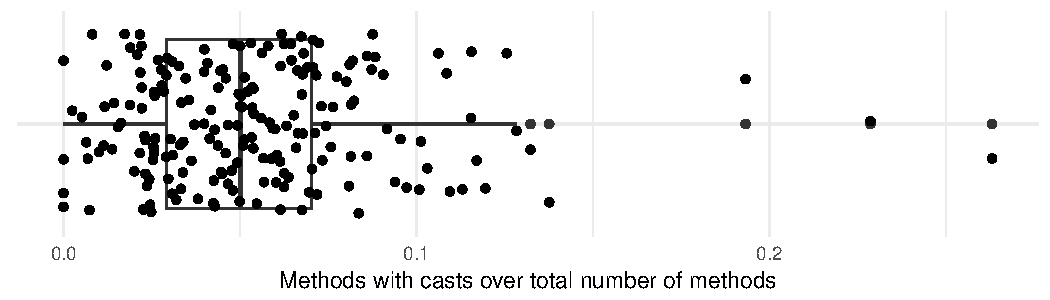
\includegraphics[width=0.9\columnwidth]{analysis/stats-methodwcastXproject.pdf}

All projects have less than 10\% of methods with at least a cast.
Overall, around a \castpercentage{}\% of methods contain at least one cast operation. 
This means there is a low density of casts.
Given the fact that generics were introduced \java{} 5, this can explain this low density.

Nevertheless, casts are still used.
We want to understand why there are casts instances (\ref{casts:rq2}) and how often the use cases that leads to casts are used (\ref{casts:rq3}).
The following sections give an answer to these questions.

% DONE: cut
% The query to gather this statistics is available online.\footnote{\url{https://gitlab.com/acuarica/java-cast-queries/blob/master/ql/stats.ql}}
% The \lang{R} script to further analyze the query results is available online as well.\footnote{\url{https://gitlab.com/acuarica/java-cast-queries/blob/master/analysis/stats.r}}

\section{Finding Casts Usage Patterns}
\label{sec:casts:methodology}

To answer both research questions
\ref{casts:rq2} (\emph{\crqB}) and \ref{casts:rq3} (\emph{\crqC})
we have used the \ql{} query language within the \lgtm{} service to look for cast instances.
%
As mentioned in section \ref{sec:casts:stats}, \ql{} treats primitive conversions as casts.
Thus, a preliminary step is to exclude them as cast instances.
The following \ql{} query shows how to retrieve all relevant cast expressions:

\begin{lstlisting}[style=ql,caption=\ql{} query to retrieve all relevant cast expressions.]
import java
from CastExpr ce where not (
ce.getExpr().getType() instanceof PrimitiveType and
ce.getTypeExpr().getType() instanceof PrimitiveType
) select ce
\end{lstlisting}

\tikzstyle{decision} = [diamond, aspect=2, draw, fill=blue!20, 
    text width=6em, text badly centered, node distance=3cm, inner sep=0pt]
\tikzstyle{block} = [rectangle, draw, fill=blue!20, 
    text width=7em, text centered, rounded corners, minimum height=2em]
\tikzstyle{block2} = [rectangle, draw, fill=blue!20, 
    text width=4.0em, text centered, rounded corners, minimum height=2em]
\tikzstyle{line} = [draw, -latex']
\tikzstyle{cloud} = [draw, ellipse,fill=red!20, node distance=3.1cm,
    minimum height=2.9em]

\begin{figure}
% \begin{wrapfigure}{r}{7.6cm}
\centering
\begin{tikzpicture}[node distance = 1.5cm, auto]
    % Place nodes
    \node [block] (run) {Run Query};
    % \node [cloud, left of=run] (tags) {Tags};
    \node [cloud, right of=run] (patterns) {Patterns};
    \node [block, below of=run] (inspect) {Inspect Casts without Pattern};
    % \node [decision, below of=inspect, node distance=1.6cm] (tag) {New Tag?};
    \node [decision, below of=inspect, node distance=2.0cm] (pattern) {New Pattern?};
    % \node [block2, left of=tag, node distance=3.1cm] (update-tags) {Update Tags};
    \node [block2, right of=pattern, node distance=3.1cm] (update-pattern) {Update Patterns};
    % \node [decision, below of=evaluate] (decide) {is best candidate better?};
    \node [block, below of=pattern, node distance=1.6cm] (stop) {Stop};
    % Draw edges
    \path [line] (run) -- (inspect);
    % \path [line] (inspect) -- (evaluate);
    % \path [line] (inspect) -- (tag);
    \path [line] (inspect) -- (pattern);
    % \path [line] (tag) -- node [near start] {yes} (update-tags);
    \path [line] (pattern) -- node [near start] {yes} (update-pattern);
    % \path [line] (update-tags) -- (tags);
    \path [line] (update-pattern) -- (patterns);
    % \path [line] (tag) -- node {no}(pattern);
    \path [line] (pattern) -- node {no}(stop);
    % \path [line,dashed] (tags) -- (run);
    \path [line,dashed] (patterns) -- (run);
\end{tikzpicture}
\caption{Process to discover cast tags and patterns.} \label{fig:process}
\end{figure}

Figure~\ref{fig:process} depicts our methodology.
We have used this initial result as a starting point for our analysis.
Afterwards, we select a random sample for manual inspection.
We manually inspected the mentioned casts trying to understand
why and how they were used.

By manually inspecting several casts instances,
we observe that certain characteristics appear often, \eg,
a cast in a overridden method, or a cast guarded by an \code{instanceof}.
We then \emph{tag} cast instances based on these observations.
We implement a \ql{} predicate that detects them and proceed
to refine our query with this new tag predicate.
% The table of tags is presented in table~\ref{table:tags}.
After a new tag is added, the query is run again to iterate over the new results.

% DONE: Remove randomly.
% Whenever we observe that those tags do not appear randomly,
Whenever we detect that those tags appear often,
we further inspect the source code to check that is indeed a pattern.
We have formalized the structure of each pattern as a \ql{} predicate based on those tags.
Similarly with tags, after a new pattern is added,
the query is run again to inspect the casts without pattern.
To sum up, our methodology iterates over the results until
no \emph{more} patterns can be detected.
% These patterns are presented in the following section.
The final \ql{} query is available online.%
\footnote{\url{https://gitlab.com/acuarica/java-cast-queries/blob/master/obs.ql}}


% DONE: What about patterns we can't write queries for?
\subsection*{Manual Categorization of Patterns}

Some code patterns might be too difficult to
express in terms of \ql{} queries.
This situation arises when the knowledge to determine
the pattern is outside the source code,
\eg, in configuration files or library call sites.
Thus, in those cases we can only acknowledge that a pattern exists,
but not how recurrent it is.

\section{Methodology}

As for the project selection, I have used the lgtm.com project database.
We can argue that this provide a good filter of projects,
since teams that want their code to be analyzed push their projects onto lgtm.com.
This will filter out for instance student projects from github.
There are also popular projects, e.g., gradle, neo4j, google guava,
that probably were pulled in by the Semmle people.
We need to double check with them, but if that’s the case,
we can make a good argument as for the project selection.

There is a total of $7.559$ projects, with a total 10,193,435 casts.
For each cast, I have the path within the project.
But to manually analyze them, I need to get the lgtm.com link.
This is necessary to actually see the code snippet in which the cast appear.
There are 215 projects for which I can’t get the lgtm.com link.
These 215 projects contains 1,162,583 casts.
There are also 516 projects which does not contain any cast.
Therefore the cast population from where make the sampling consists of
9,030,852 casts spread in 6,840 projects.

Now comes the question: What is an appropriate sample size?
Using this online calculator:

https://www.surveysystem.com/sscalc.htm

With standard parameters, Confidence Level=95\% and Confidence Interval=5,
I got a sample size of 384.
This seems sketchy.
My first approach was to increase the sample size arbitrarily,
e.g., 10,000 casts to manually analyze.
This can be too much effort.
But more importantly, how to come up with the patterns taxonomy?
The current list of patterns I have (using QL) does not cover all
existing patterns, i.e.,
when doing manual sample I have discovered new patterns.
After meeting with Gabriele, he suggested using saturation sampling:
0. Start with an empty list of patterns.
1. Perform a manual sample of, let’s say 384 casts.
2. For each new pattern seen, add it to the list of patterns.
3. If a new pattern is detected, go to step 1.

\section{Cast Usage Patterns}
\label{sec:patterns}

Using the methodology described in the above section, we have devised \npattern{} casts usage patterns.%
\footnote{We have excluded casts that represents primitive numeric type conversions, as they do not represent any pattern.
However, during our manual analysis we found \nprim{} primitive conversions.
Moreover, we found \nbrokenlinks{} links that were not accessible during our analysis.}
In this section we present the cast usage patterns we found.
To ease the patterns presentation, we have clustered them in \ngroup{} groups according to their purpose.
Figure~\ref{fig:patterns} shows our patterns and their occurrences sort by frequency.
The column on the right correspond to the group the pattern belongs to.

\begin{figure}[ht!]
\centering
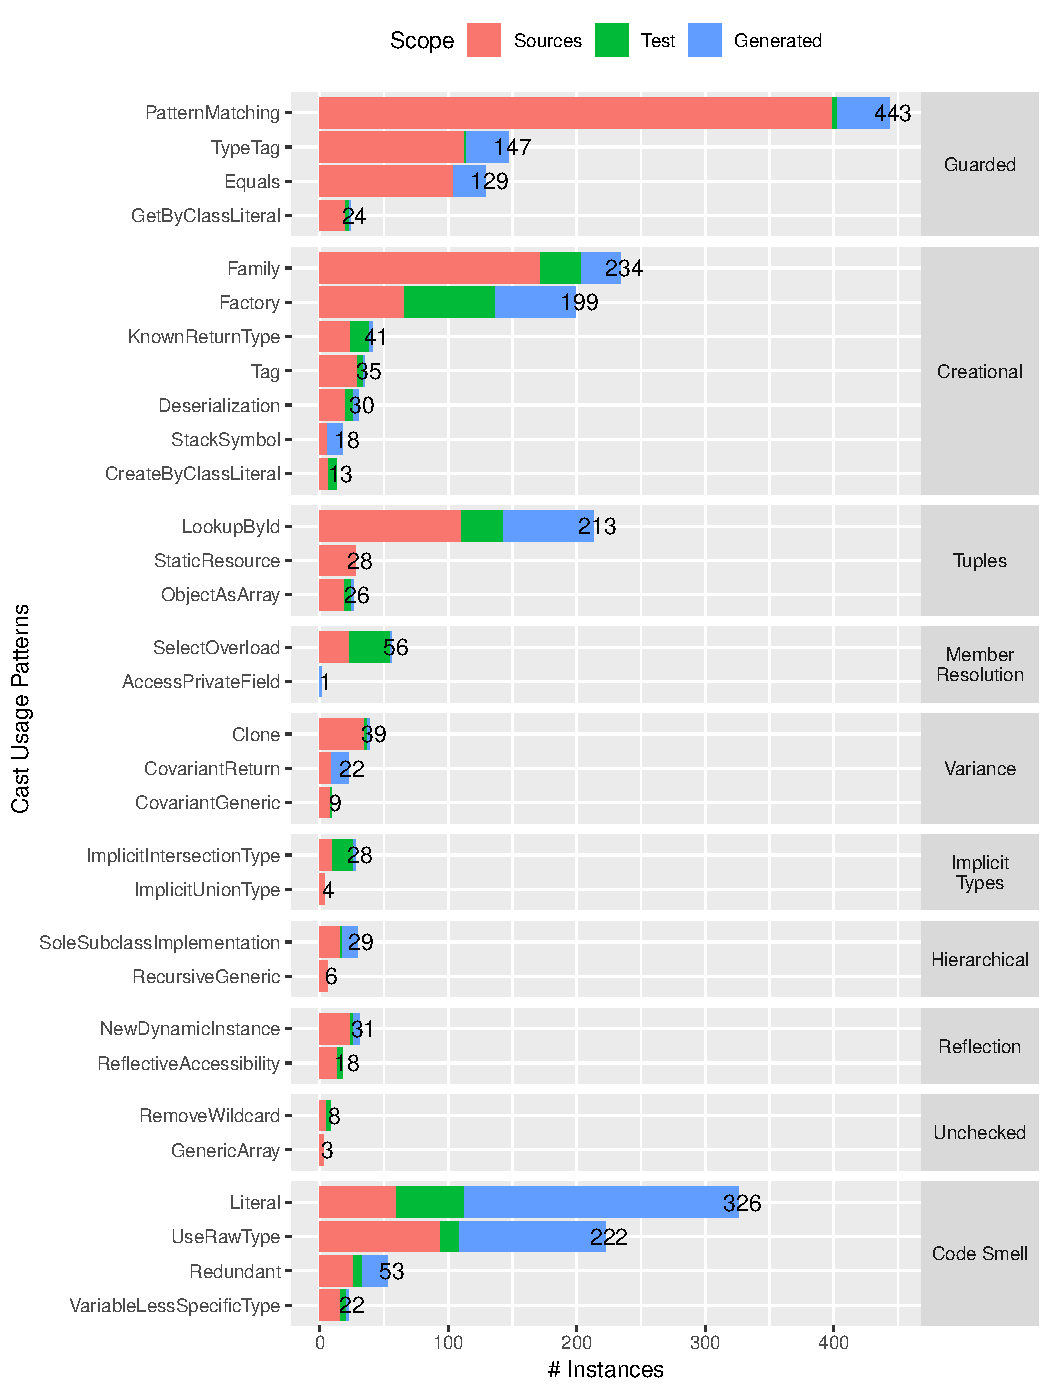
\includegraphics[width=\textwidth]{analysis/table-patterns-5000.pdf}
\caption{Cast Patterns Occurrences} \label{fig:patterns}
\end{figure}

Each pattern is described using the following template:

\begin{itemize}
\item \textbf{Description.}
Tells what is this pattern about.
It gives a general overview of the structure of the pattern.
\item \textbf{Instances.}
Gives one or more concrete examples found in real code.%
\footnote{Please notice that the snippets presented here were slightly
modified for formatting purposes.
Moreover, to facilitate some snippet presentations,
we remove irrelevant code and replace it with the
comment \code{// [...]}.}
For each instance presented here, we provide the link to the source code repository in \lgtm{}.
We provide the link in case the reader wants to do further inspection
of the snippet presented.%
\footnote{Instead of presenting \lgtm{} long URLs,
we have used the URL shortening service \url{https://bitly.com/}
for an easier reading.}
\item \textbf{Detection.}
Describes briefly how this pattern was detected in terms of the tags introduced in the previous section.
\item \textbf{Discussion.}
Presents suggestions, flaws, or comments about the pattern.
\item \textbf{Related Patterns.}
How the pattern being described relates to other patterns?
\end{itemize}

\group{Guarded}

The patterns in this group are guarded casts.


\begin{pattern}{PatternMatching}
This pattern is composed of a guard (\code{instanceof}) followed by a
cast on known subtypes of the static type.
Often there is just one case and the default case, \ie,
\code{instanceof} fails, does a no-op or reports an error.
Another common approach is to have several cases,
usually one \emph{per} subtype.

\instances{}
The following listing shows an example of the \thisp{} pattern.%
\footnote{\url{http://bit.ly/2FzYYHq}}
In this example, there is only one case

% https://lgtm.com/projects/g/OpenMods/OpenBlocks/snapshot/dist-2040060754-1524814812150/files/build/sources/java/openblocks/common/tileentity/TileEntityImaginary.java?sort=name&dir=ASC&mode=heatmap#L268
\begin{minted}[highlightlines=3]{java}
Item item = helmet.getItem();
if (item instanceof ItemImaginationGlasses)
	return ((ItemImaginationGlasses)item).checkBlock(what, helmet, this);
\end{minted}

Double typecase example
\footnote{\url{http://bit.ly/2FDN9Rd}}

% https://lgtm.com/projects/g/bbossgroups/bboss/snapshot/dist-2025970729-1524814812150/files/bboss-util/src/org/frameworkset/util/ObjectUtils.java?sort=name&dir=ASC&mode=heatmap#L228
\begin{minted}[highlightlines=25]{java}
public static boolean nullSafeEquals(Object o1, Object o2) {
	if (o1 == o2) {
		return true;
	}
	if (o1 == null || o2 == null) {
		return false;
	}
	if (o1.equals(o2)) {
		return true;
	}
	if (o1.getClass().isArray() && o2.getClass().isArray()) {
		if (o1 instanceof Object[] && o2 instanceof Object[]) {
			return Arrays.equals((Object[]) o1, (Object[]) o2);
		}
		if (o1 instanceof boolean[] && o2 instanceof boolean[]) {
			return Arrays.equals((boolean[]) o1, (boolean[]) o2);
		}
		if (o1 instanceof byte[] && o2 instanceof byte[]) {
			return Arrays.equals((byte[]) o1, (byte[]) o2);
		}
		if (o1 instanceof char[] && o2 instanceof char[]) {
			return Arrays.equals((char[]) o1, (char[]) o2);
		}
		if (o1 instanceof double[] && o2 instanceof double[]) {
			return Arrays.equals((double[]) o1, (double[]) o2);
		}
		if (o1 instanceof float[] && o2 instanceof float[]) {
			return Arrays.equals((float[]) o1, (float[]) o2);
		}
		if (o1 instanceof int[] && o2 instanceof int[]) {
			return Arrays.equals((int[]) o1, (int[]) o2);
		}
		if (o1 instanceof long[] && o2 instanceof long[]) {
			return Arrays.equals((long[]) o1, (long[]) o2);
		}
		if (o1 instanceof short[] && o2 instanceof short[]) {
			return Arrays.equals((short[]) o1, (short[]) o2);
		}
	}
	return false;
}
\end{minted}


\detection{}
To detect this pattern, we look

\discussion{}
The \thisp{} pattern can be seen as an \adhoc{}
alternative to pattern matching.
This construct can be seen in several other languages, \eg,
\haskell{}, \scala{}, and \cs{}.
There is an ongoing proposal%
\footnote{\url{http://openjdk.java.net/jeps/305}} to add pattern
matching to the \java{} language.

As a workaround, alternatives to the \thisp{} pattern can be the
visitor pattern or polymorphism.
But in some cases, the chain of \code{instanceof}s is of boxed types.
Thus no polymorphism can be used.

% Maybe this should be called properly instanceof-guarded cast, to be more specific.
% This pattern checks whether a parameter in an overridden method has a more specific type.
% A cast to a variable guarded by an \code{instanceof}.
% A variable is \emph{guarded} by a condition when the condition controls
% that access to the variable, and there is no assignment after the
% condition and before the access to that variable.

The \thisp{} pattern consists of testing the runtime type of a variable against several related types.
Based on rule taken from:
It was taken from a \lgtm{} rule\footnote{\url{https://lgtm.com/rules/910065/}}.

It is a technique that allows a developer to take different actions according to the runtime type of an object.
Depending on the --- runtime --- type of an object, different cases, usually one for each type will follow.

\end{pattern}

\begin{pattern}{TypeTag}
%
\done{Matthias: Your first example doesn't have the tag in the *same* object, but passes it as a separate variable.}
%
A cast instance belonging to the \thisp{} pattern is guarded by an application-specific test instead of using an \code{instanceof} test.

\instances{}
The following example%
\footnote{\url{http://bit.ly/JesusFreke_smali_2Ho8bVL}}
shows an instance of the \thisp{} pattern.
The cast type of the parameter \code{reference} is determined by the value of the parameter \code{referenceType}.

%https://lgtm.com/projects/b/JesusFreke/smali/snapshot/dist-1306230039-1524814812150/files/dexlib2/src/main/java/org/jf/dexlib2/writer/InstructionWriter.java?sort=name&dir=ASC&mode=heatmap#L492
\begin{minted}[highlightlines=8]{java}
private int getReferenceIndex(int referenceType, Reference reference) {
    switch (referenceType) {
        case ReferenceType.FIELD:
            return fieldSection.getItemIndex((FieldRefKey) reference);
        case ReferenceType.METHOD:
            return methodSection.getItemIndex((MethodRefKey) reference);
        case ReferenceType.STRING:
            return stringSection.getItemIndex((StringRef) reference);
        case ReferenceType.TYPE:
            return typeSection.getItemIndex((TypeRef) reference);
        case ReferenceType.METHOD_PROTO:
            return protoSection.getItemIndex((ProtoRefKey) reference);
        default:
            throw new ExceptionWithContext(
                "Unknown reference type: %d",  referenceType);
    }
}
\end{minted}

In the next example,%
\footnote{\url{http://bit.ly/FenixEdu_fenixedu-academic_2SUNOUJ}}
instead of a \code{switch} statement,
an \code{if} statement is used to guard the cast (in line 6).

%https://lgtm.com/projects/g/FenixEdu/fenixedu-academic/snapshot/dist-29270029-1524814812150/files/src/main/java/org/fenixedu/academic/ui/renderers/student/curriculum/StudentCurricularPlanRenderer.java?sort=name&dir=ASC&mode=heatmap#L853
\begin{minted}[highlightlines=6]{java}
for (final IEnrolment enrolment : dismissal.getSourceIEnrolments()) {
    if (enrolment.isExternalEnrolment()) {
        generateExternalEnrolmentRow(mainTable, (ExternalEnrolment) enrolment,
                level + 1, true);
    } else {
        generateEnrolmentRow(mainTable, (Enrolment) enrolment,
                level + 1, false, true, true);
    }
}
\end{minted}

\done{Nate: Why is this not pattern matching?}
%
In the next case%
\footnote{\url{http://bit.ly/apache_poi_2FW5SXU}}
a type test is performed --- through a method call --- before actually applying the cast to the variable \code{props} (line 3).
Note that the type test is internally using the \code{instanceof} operator (line 8).
Although in this case the type test is using an \code{instanceof} operator,
it is not considered \nameref{pat:PatternMatching} because the \code{instanceof} is located in a method call.

%https://lgtm.com/projects/g/apache/poi/snapshot/dist-1790760597-1524814812150/files/src/ooxml/java/org/apache/poi/xslf/usermodel/XSLFPropertiesDelegate.java?sort=name&dir=ASC&mode=heatmap#L1367
\begin{minted}[highlightlines=3]{java}
@Override
public CTSolidColorFillProperties getSolidFill() {
    return isSetSolidFill() ? (CTSolidColorFillProperties)props : null;
}

@Override
public boolean isSetSolidFill() {
    return (props instanceof CTSolidColorFillProperties);
}
\end{minted}

In some cases, the type to be casted to is the same in every branch.
The following snippet%
\footnote{\url{http://bit.ly/loopj_android-async-http_2IpIULk}}
shows an instance of this case.
The cast is applied to the \code{message.obj} field to (line 13),
according to the value of the \code{message.what} field (line 1).
However, a similar cast is applied in the first branch (line 3).
In both branches \code{message.obj} is of type \code{Object[]},
but in the case of \code{FAILURE\_MESSAGE},
the array contains one more element (line 16).
This suggests that the \code{(Object[]) message.obj} array denotes two different objects,
but are not distinguishable from the type system perspective.

%https://lgtm.com/projects/g/loopj/android-async-http/snapshot/dist-1879340034-1549372228293/files/library/src/main/java/com/loopj/android/http/AsyncHttpResponseHandler.java?sort=name&dir=ASC&mode=heatmap#L359
\begin{minted}[highlightlines=13]{java}
switch (message.what) {
    case SUCCESS_MESSAGE:
        response = (Object[]) message.obj;
        if (response != null && response.length >= 3) {
            onSuccess((Integer) response[0], (Header[]) response[1],
                    (byte[]) response[2]);
        } else {
            AsyncHttpClient.log.e(LOG_TAG, 
                    "SUCCESS_MESSAGE didn't got enough params");
        }
        break;
    case FAILURE_MESSAGE:
        response = (Object[]) message.obj;
        if (response != null && response.length >= 4) {
            onFailure((Integer) response[0], (Header[]) response[1],
                    (byte[]) response[2], (Throwable) response[3]);
        } else {
            AsyncHttpClient.log.e(LOG_TAG,
                    "FAILURE_MESSAGE didn't got enough params");
        }
        break;
    // [...]
}
\end{minted}


\detection{}
The detection of this pattern is similar to the \nameref{pat:PatternMatching} detection, but instead of looking for an \code{instanceof} guarded cast, we look for an application-specific guard.
The guard needs to determine either the resulting type of the cast instance, or
the subsequent operations applied to the result of the cast instance if the types in every branch are the same.

\discussion{}
In some cases, the \thisp{} pattern can be replaced by \nameref{pat:PatternMatching}.
However, if the application-specific tag is a numeric value,
the \thisp{} could perform better than the \nameref{pat:PatternMatching} using \code{instanceof}.
Moreover, there are situation where the \thisp{} can not be avoid since the types to be casted to are the same.

\related{}
%
\done{Nate: PatternMatching}
This pattern is related to \nameref{pat:PatternMatching} since both denoted guarded casts.
The difference is that \thisp{} uses an application-specific test.
\nameref{pat:GetByClassLiteral} could be seen as a special case of \thisp{} where the tag is a class literal.

\end{pattern}
\begin{pattern}{Equals}
This pattern is a common pattern to implement the \code{equals} method (declared in \code{java.lang.Object}).
A cast expression is guarded by either an \code{instanceof} test or a \code{getClass} comparison (usually to the same target type as the cast);
in an \code{equals}%
\footnote{\url{https://docs.oracle.com/javase/8/docs/api/java/lang/Object.html\#equals-java.lang.Object-}} method implementation.
This is done to check if the argument has same type as the receiver
(\code{this} argument).

Notice that a cast in an \code{equals} method is needed because it
receives an \code{Object} as a parameter.

\instances{}
The following listing%
\footnote{\url{http://bit.ly/neo4j_neo4j_2vJw94J}}
shows an example of the \pname{} pattern.
In this case,
\code{instanceof} is used to guard for the same type as the receiver.

%https://lgtm.com/projects/g/neo4j/neo4j/snapshot/dist-15760049-1519892555006/files/community/kernel/src/main/java/org/neo4j/kernel/impl/api/CountsRecordState.java?sort=name&dir=ASC&mode=heatmap&excluded=false#L182
\begin{minted}[highlightlines=7]{java}
@Override
public boolean equals(Object obj) {
    if ( this == obj ) {
        return true;
    }
    if ( (obj instanceof Difference) ) {
        Difference that = (Difference) obj;
        return actualFirst == that.actualFirst
          && expectedFirst == that.expectedFirst
          && actualSecond == that.actualSecond 
          && expectedSecond == that.expectedSecond
          && key.equals( that.key );
    }
    return false;
}
\end{minted}

Alternatively, the following listing%
\footnote{\url{http://bit.ly/neo4j_neo4j_2vKP0MW}}
shows another example of the \thisp{} pattern.
But in this case,
a \code{getClass} comparison is used to guard for the same type as the receiver.

%https://lgtm.com/projects/g/neo4j/neo4j/snapshot/dist-15760049-1519892555006/files/community/bolt/src/main/java/org/neo4j/bolt/v1/messaging/infrastructure/ValuePath.java?sort=name&dir=ASC&mode=heatmap&excluded=false#L278
\begin{minted}[highlightlines=7]{java}
@Override
public boolean equals( Object o ) {
    if ( this == o ) return true;
    if ( o == null || getClass() != o.getClass() )
        return false;

    ValuePath that = (ValuePath) o;
    return nodes.equals(that.nodes) &&
        relationships.equals(that.relationships);
}
\end{minted}

In some situations, the type casted to is not same as the enclosing class.
Instead, the type casted to is the super class of the enclosing class.
The following example%
\footnote{\url{http://bit.ly/square_sqlbrite_2HmHMYE}}
shows this scenario.
This usually happens when the Google AutoValue library%
\footnote{\url{https://github.com/google/auto/tree/master/value}}
is used.
The AutoValue is a code generator for value classes.

%https://lgtm.com/projects/g/square/sqlbrite/snapshot/3a9916985485ba5922097fe59a18230500f02df4/files/sample/build/generated/source/apt/debug/com/example/sqlbrite/todo/ui/$AutoValue_ListsItem.java?sort=name&dir=ASC&mode=heatmap&showExcluded=false#L52
\begin{minted}[highlightlines=13]{java}
@AutoValue
abstract class ListsItem implements Parcelable {
    // [...]
}

abstract class $AutoValue_ListsItem extends ListsItem {
    @Override
    public boolean equals(Object o) {
      if (o == this) {
        return true;
      }
      if (o instanceof ListsItem) {
        ListsItem that = (ListsItem) o;
        return (this.id == that.id())
             && (this.name.equals(that.name()))
             && (this.itemCount == that.itemCount());
      }
      return false;
    }
}
\end{minted}

The following shows a non-trivial implementation of equals.
\footnote{\url{http://bit.ly/bndtools_bnd_2SM5pOw}}

%https://lgtm.com/projects/g/bndtools/bnd/snapshot/dist-930051-1524814812150/files/biz.aQute.bndlib/src/aQute/bnd/osgi/resource/CapReq.java?sort=name&dir=ASC&mode=heatmap#L73
\begin{minted}[highlightlines=12]{java}
@Override
public boolean equals(Object obj) {
    if (this == obj)
            return true;
    if (obj == null)
            return false;
    if (obj instanceof CapReq)
            return equalsNative((CapReq) obj);
    if ((mode == MODE.Capability) && (obj instanceof Capability))
            return equalsCap((Capability) obj);
    if ((mode == MODE.Requirement) && (obj instanceof Requirement))
            return equalsReq((Requirement) obj);
    return false;
}
\end{minted}

\detection{}
The detection query looks for a cast expression inside an \code{equals} method implementation.
Moreover, the cast needs to be guarded by either an \code{instanceof} test or a \code{getClass} comparison.
And the type being casted to needs to be either the same as the enclosing class or a superclass of it.

\discussion{}
The pattern for an \code{equals} method implementation is well-known.

We found out that, with respect to cast,
most \code{equals} methods are implemented with the same structure.
Maybe avoid boilerplate code by providing code generation,
%
\todo{Nate: \rust{} traits too. \code{\#[derive(Eq)]} }
%
like in \haskell{} (with \code{deriving}).

\cite{vaziriDeclarativeObjectIdentity2007} propose a declarative approach to avoid boilerplate code when implementing both the \code{equals} and \code{hashCode} methods.
They manually analyzed several applications, and found there are many issues while implementing \code{equals()} and \code{hashCode()} methods.
It would be interesting to check whether these issues happen in real application code.

There is an exploratory document%
\footnote{\url{http://cr.openjdk.java.net/\~briangoetz/amber/datum.html}}
by Brian Goetz --- \java{} Language Architect --- addressing these issues from a more general perspective.
It is definitely a starting point towards improving the \java{} language.

\related{}
This pattern can be seen as a special instance of the \nameref{pat:PatternMatching} pattern.
\end{pattern}
\begin{pattern}{GetByClassLiteral}
A cast is using an application-specific guard,
but the guard depends on a class literal.

\instances{}
The following example,%
\footnote{\url{http://bit.ly/elastic_elasticsearch_2SSgsFV}}
shows an instance of the \thisp{} pattern.
A cast is performed to the \code{field} variable (line 22),
based whether the runtime class of the variable is actually \code{Short.class}.

%https://lgtm.com/projects/g/elastic/elasticsearch/snapshot/dist-1916470085-1524814812150/files/server/src/main/java/org/elasticsearch/common/lucene/Lucene.java?sort=name&dir=ASC&mode=heatmap#L478
\begin{minted}[highlightlines=22]{java}
Class type = field.getClass();
if (type == String.class) {
    out.writeByte((byte) 1);
    out.writeString((String) field);
} else if (type == Integer.class) {
    out.writeByte((byte) 2);
    out.writeInt((Integer) field);
} else if (type == Long.class) {
    out.writeByte((byte) 3);
    out.writeLong((Long) field);
} else if (type == Float.class) {
    out.writeByte((byte) 4);
    out.writeFloat((Float) field);
} else if (type == Double.class) {
    out.writeByte((byte) 5);
    out.writeDouble((Double) field);
} else if (type == Byte.class) {
    out.writeByte((byte) 6);
    out.writeByte((Byte) field);
} else if (type == Short.class) {
    out.writeByte((byte) 7);
    out.writeShort((Short) field);
} else if (type == Boolean.class) {
    out.writeByte((byte) 8);
    out.writeBoolean((Boolean) field);
} else if (type == BytesRef.class) {
    out.writeByte((byte) 9);
    out.writeBytesRef((BytesRef) field);
} else {
    throw new IOException("Can't handle sort field value of type ["+type+"]");
}
\end{minted}

\detection{}

\discussion{}

\related{}

\end{pattern}
\begin{pattern}{ClassForName}

\instances{}

\detection{}

\discussion{}

\related{}

\end{pattern}

\group{Creational}

These patterns creates to how they are created.

\begin{pattern}{Family}
Family polymorphism.

\instances{}

\begin{minted}[highlightlines=1]{java}
\end{minted}

\detection{}

\discussion{}
\cite{ernstFamilyPolymorphism2001}

\related{}

\end{pattern}
\begin{pattern}{Factory}
\todo{Also Logger}
Creates an object based on some arguments either to the method call or constructor.
Since the arguments are known at compile-time, cast to the specific type.

\todo{Nate: Move to "Related Patterns"}
Cast factory method result to subtype (special case of family polymorphism).
Usually Logger.getLogger.

The method is declared to return URLConnection but can return a more specific type based on the URL string.
Cast to that.
We should generalize this pattern.
%
\todo{Nate: Create with type descriptor "Tag"}

\instances{}
\todo{Describe}
\footnote{\url{http://bit.ly/connect2id_oauth-2-0-sdk-with-_2HvRlUX}}

\footnote{\url{https://docs.oracle.com/javase/8/docs/api/java/security/KeyPair.html\#getPrivate()}}

%https://lgtm.com/projects/b/connect2id/oauth-2.0-sdk-with-openid-connect-extensions/snapshot/dist-1311020143-1524814812150/files/src/test/java/com/nimbusds/oauth2/sdk/jose/jwk/RemoteJWKSetTest.java?sort=name&dir=ASC&mode=heatmap#L242
\begin{minted}[highlightlines=10]{java}
KeyPairGenerator pairGen = KeyPairGenerator.getInstance("RSA");
pairGen.initialize(1024);
KeyPair keyPair = pairGen.generateKeyPair();
RSAKey rsaJWK1 = new RSAKey.Builder((RSAPublicKey) keyPair.getPublic())
        .privateKey((RSAPrivateKey) keyPair.getPrivate())
        .keyID("1")
        .build();
keyPair = pairGen.generateKeyPair();
RSAKey rsaJWK2 = new RSAKey.Builder((RSAPublicKey) keyPair.getPublic())
        .privateKey((RSAPrivateKey) keyPair.getPrivate())
        .keyID("2")
        .build();
\end{minted}

\done{Also URLOpenConnection.}
\footnote{\url{http://bit.ly/apache_hadoop_2E6KY6T}}

\footnote{\url{https://docs.oracle.com/javase/8/docs/api/java/net/URL.html\#openConnection--}}

%https://lgtm.com/projects/g/apache/hadoop/snapshot/dist-956730001-1524814812150/files/hadoop-yarn-project/hadoop-yarn/hadoop-yarn-server/hadoop-yarn-server-resourcemanager/src/test/java/org/apache/hadoop/yarn/server/resourcemanager/webapp/TestRMWebServicesHttpStaticUserPermissions.java?sort=name&dir=ASC&mode=heatmap#L138
\begin{minted}[highlightlines=2]{java}
URL url = new URL("http://localhost:8088/ws/v1/cluster/apps");
HttpURLConnection conn = (HttpURLConnection) url.openConnection();
\end{minted}

\detection{}

\discussion{}

\related{}

\end{pattern}
\begin{pattern}{KnownLibraryMethod}
There are cases when a method's return type is less specific than the
actual return type value.
This is usually to hide implementation details.
Nevertheless, sometimes it is convenient for the developer to work
directly on the actual return type.
This pattern is used to cast from the method's return type to
the \emph{known} actual return type.

\instances{}

\footnote{\url{}}

\begin{minted}[highlightlines=1]{java}

\end{minted}

\detection{}

\discussion{}

\related{}

\end{pattern}
\begin{pattern}{NewDynamicInstance}
%
\todo{Nate: Why not Creational?}
%
Dynamically creates an object or array by means of reflection.
The \code{newInstance} method family declared in the \code{Class},%
\footnote{\url{https://docs.oracle.com/javase/8/docs/api/java/lang/Class.html\#newInstance--}}
\code{Array}\footnote{\url{https://docs.oracle.com/javase/8/docs/api/java/lang/reflect/Array.html\#newInstance-java.lang.Class-int-}}\(^{,}\)
\footnote{\url{https://docs.oracle.com/javase/8/docs/api/java/lang/reflect/Array.html\#newInstance-java.lang.Class-int...-}}
and \code{Constructor}%
\footnote{\url{https://docs.oracle.com/javase/8/docs/api/java/lang/reflect/Constructor.html\#newInstance-java.lang.Object...-}}
classes creates an object or array dynamically by means of reflection, \ie, the type of object being created is not known at compile-time.
This pattern consists of casting the result of these methods to the appropriate target type.

\instances{}
The following example%
\footnote{\url{http://bit.ly/2HC3IPg}}
shows a cast to the \code{Class.newInstance()}
method.

%https://lgtm.com/projects/g/apache/hadoop/snapshot/6bedbef6c5f2d937a6cbc268300ce2a39609d06c/files/hadoop-hdfs-project/hadoop-hdfs/src/main/java/org/apache/hadoop/hdfs/server/namenode/FSNamesystem.java?sort=name\&dir=ASC\&mode=heatmap\&showExcluded=false#L1039
\begin{minted}[highlightlines=1]{java}
logger = (AuditLogger) Class.forName(className).newInstance();
\end{minted}

The following example%
\footnote{\url{http://bit.ly/2Hp5Hqc}}
shows how to dynamically create an array, using the \texttt{Array} class.

%https://lgtm.com/projects/g/neo4j/neo4j/snapshot/27aaa67633e4d26446e38125d04fbbd27f938b75/files/community/collections/src/main/java/org/neo4j/helpers/collection/Iterables.java?sort=name\&dir=ASC\&mode=heatmap\&showExcluded=false#L403
\begin{minted}[highlightlines=1]{java}
return list.toArray( (T[]) Array.newInstance( componentType, list.size()));
\end{minted}

Whenever a constructor other than the default constructor is needed,
the \code{newInstance} method declared in the \code{Constructor} class
should be used to select the appropriate constructor,
as shown in the following example.
\footnote{\url{http://bit.ly/2HsUgOo}}

%https://lgtm.com/projects/g/gradle/gradle/snapshot/209c3175e75af6ac30cb66c02eda15b0f8b6a616/files/subprojects/internal-integ-testing/src/main/groovy/org/gradle/integtests/fixtures/executer/OutputScrapingExecutionFailure.java?sort=name\&dir=ASC\&mode=heatmap\&showExcluded=false#L174
\begin{minted}[highlightlines=1]{java}
return (Exception) Class
                       .forName(className)
                       .getConstructor(String.class)
                       .newInstance(message);
\end{minted}

The following example%
\footnote{\url{http://bit.ly/2HC33xg}}
shows a guarded instance of the \thisp{} pattern.
This seems rather unusual, as this pattern is not guarded.

%https://lgtm.com/projects/g/alibaba/LuaViewSDK/snapshot/dist-2037250419-1524814812150/files/Android/LuaViewSDK/src/com/taobao/luaview/global/LuaViewManager.java?sort=name&dir=ASC&mode=heatmap#L373
\begin{minted}[highlightlines=6]{java}
private static List<String> getMapperMethodNames(final Class clazz) {
    try {
        if (clazz != null) {
            Object obj = clazz.newInstance();
            if (obj instanceof BaseMethodMapper) {
                return ((BaseMethodMapper) obj).getAllFunctionNames();
            }
        }
    } catch (Exception e) {
        e.printStackTrace();
    }
    return null;
}
\end{minted}

There are cases when the cast is not directly applied to the result of the \code{newInstance} method.
The following snippet shows such a case.%
\footnote{\url{http://bit.ly/2HJtXUn}}
The cast is used to convert from \code{Class<?>} to \code{Class<ConfigFactory>} (line 4).
The \code{newInstance} invocation then does not need a direct cast (line 8) given the definition of the \code{clazz} variable (line 2).
Nevertheless, the cast is unchecked, and a \code{checkcast} instruction is going to be emitted anyway for the result of the \code{newInstance} invocation.

%https://lgtm.com/projects/g/pac4j/pac4j/snapshot/dist-4840350-1524814812150/files/pac4j-core/src/main/java/org/pac4j/core/config/ConfigBuilder.java?sort=name&dir=ASC&mode=heatmap#L25
\begin{minted}[highlightlines=4]{java}
ClassLoader tccl = Thread.currentThread().getContextClassLoader();
final Class<ConfigFactory> clazz;
if (tccl == null) {
    clazz = (Class<ConfigFactory>) Class.forName(factoryName);
} else {
    clazz = (Class<ConfigFactory>) Class.forName(factoryName, true, tccl);
}
final ConfigFactory factory = clazz.newInstance();
\end{minted}


\detection{}
This detection query looks for casts,
where the expression being cast is a call site to methods mentioned above.

\discussion{}
The cast here is needed because of the dynamic essence of reflection.
This pattern is mostly unguarded, that is,
the application programmer knows what target type is being created.

The following two code snippets:

\begin{minted}{java}
Class<?> c = Class.forName("java.lang.String");
String pf = (String) c.newInstance();
\end{minted}

\begin{minted}{java}
Class<String> c = (Class<String>) Class.forName("java.lang.String");
String pf = c.newInstance();
\end{minted}

compile to the same bytecode below.

\begin{lstlisting}[style=bytecode]
ldc           #24    // String java.lang.String
invokestatic  #26    // Method java/lang/Class.forName
astore_1
aload_1
invokevirtual #32    // Method java/lang/Class.newInstance
checkcast     #36    // class java/lang/String
\end{lstlisting}

\related{}
Reflection.

\end{pattern}
\begin{pattern}{Tag}
Used 

\instances{}

\footnote{\url{http://bit.ly/2HUmGki}}

%https://lgtm.com/projects/g/UniTime/cpsolver/snapshot/dist-4860376-1524814812150/files/src/org/cpsolver/ifs/assignment/context/AssignmentContextHolderMap.java?sort=name&dir=ASC&mode=heatmap#L47
\begin{minted}[highlightlines=9]{java}
protected Map<Integer,AssignmentContext> iContexts =
                new HashMap<Integer, AssignmentContext>();

@Override
@SuppressWarnings("unchecked")
public <U extends AssignmentContext> U getAssignmentContext(
                Assignment<V, T> assignment,
                AssignmentContextReference<V, T, U> reference) {
    U context = (U) iContexts.get(reference.getIndex());
    if (context != null) return context;
    
    context = reference.getParent().createAssignmentContext(assignment);
    iContexts.put(reference.getIndex(), context);
    return context;
}
\end{minted}

\detection{}

\discussion{}

\related{}
Related to \nameref{pat:VariableLessSpecificType}.
\nameref{pat:LookupById}.

\end{pattern}
\begin{pattern}{Deserialization}
This pattern is used to deserialize an object at run-time.

\instances{}
The following example%
\footnote{\url{http://bit.ly/internetarchive_heritrix3_2SF4j7k}}
shows how the \thisp{} pattern is used to create objects from a file system (line 19).

%https://lgtm.com/projects/g/internetarchive/heritrix3/snapshot/dist-12140105-1524814812150/files/engine/src/test/java/org/archive/crawler/datamodel/CrawlURITest.java?sort=name&dir=ASC&mode=heatmap#L83
\begin{minted}[highlightlines=19]{java}
final public void testSerialization()
        throws IOException, ClassNotFoundException {
    File serialize = new File(getTmpDir(),
            this.getClass().getName() + ".serialize");
    try {
        FileOutputStream fos = new FileOutputStream(serialize);
        ObjectOutputStream oos = new ObjectOutputStream(fos);
        oos.writeObject(this.seed);
        oos.reset();
        oos.writeObject(this.seed);
        oos.reset();
        oos.writeObject(this.seed);
        oos.close();
        // Read in the object.
        FileInputStream fis = new FileInputStream(serialize);
        ObjectInputStream ois = new ObjectInputStream(fis);
        CrawlURI deserializedCuri = (CrawlURI)ois.readObject();
        deserializedCuri = (CrawlURI)ois.readObject();
        deserializedCuri = (CrawlURI)ois.readObject();
        assertEquals("Deserialized not equal to original",
                this.seed.toString(), deserializedCuri.toString());
        String host = this.seed.getUURI().getHost();
        assertTrue("Deserialized host not null",
                host != null && host.length() >= 0);
    } finally {
        serialize.delete();
    }
}
\end{minted}

\detection{}
This pattern is characterized for a cast to the \code{readObject} method on a \code{ObjectInputStream} object.

\discussion{}
From a language design perspective,
the \thisp{} pattern is one of the most difficult patterns to avoid.
It is difficult to avoid because a compiler cannot verify at compile-time that a certain byte stream can be deserialized into an object of a given type.

\related{}
Both this pattern and the \nameref{pat:NewDynamicInstance} pattern create objects by using reflection.
\nameref{pat:StaticResource}

\end{pattern}
% \begin{pattern}{StackSymbol}

\instances{}

\footnote{\url{http://bit.ly/2HF6nrF}}

%https://lgtm.com/projects/g/fabioz/Pydev/snapshot/dist-20832102-1524814812150/files/plugins/org.python.pydev.parser/src/org/python/pydev/parser/grammar27/TreeBuilder27.java?sort=name&dir=ASC&mode=heatmap#L231
\begin{minted}[highlightlines=1]{java}
            case JJTASSERT_STMT:
                exprType msg = arity == 2 ? ((exprType) stack.popNode()) : null;
                test = (exprType) stack.popNode();
                return new Assert(test, msg);
\end{minted}

\detection{}

\discussion{}

\related{}

\end{pattern}
\begin{pattern}{CreateByClassLiteral}
    
\instances{}
\done{Nate: CreateByClassLiteral}
The following snippet\footnote{\url{http://bit.ly/apache_karaf_2HE55gE}} shows an instance of the \thisp{} pattern. 
Even if a test against a class literal (\code{AtomicInteger.class}) is used to determine a suitable cast for the parameter \code{value}.

%https://lgtm.com/projects/g/apache/karaf/snapshot/dist-13960098-1524814812150/files/shell/core/src/main/java/org/apache/karaf/shell/support/converter/DefaultConverter.java?sort=name&dir=ASC&mode=heatmap#L117
\begin{minted}[highlightlines=4]{java}
public Object convertToNumber(Number value, Class toType) throws Exception {
    toType = unwrap(toType);
    if (AtomicInteger.class == toType) {
        return new AtomicInteger((Integer)convertToNumber(value,Integer.class));
    } else if (AtomicLong.class == toType) {
        return new AtomicLong((Long) convertToNumber(value, Long.class));
    } else if (Integer.class == toType) {
        return value.intValue();
    } else if (Short.class == toType) {
        return value.shortValue();
    } else if (Long.class == toType) {
        return value.longValue();
    } else if (Float.class == toType) {
        return value.floatValue();
    } else if (Double.class == toType) {
        return value.doubleValue();
    } else if (Byte.class == toType) {
        return value.byteValue();
    } else if (BigInteger.class == toType) {
        return new BigInteger(value.toString());
    } else if (BigDecimal.class == toType) {
        return new BigDecimal(value.toString());
    } else {
        throw new Exception("Unable to convert number "+value+" to "+toType);
    }
}
\end{minted}


\detection{}

\discussion{}

\related{}

\end{pattern}

\group{Tuples}

Tuples patterns.

\begin{pattern}{LookupById}
This pattern is used to extract stashed values from a generic container.

Lookup an object by ID, tag or name and cast the result
(it is used often in Android code).
It accesses a collection that holds values of different types
(usually implemented as \code{Collection<Object>} or as \code{Map<K, Object>}).

\instances

%https://lgtm.com/projects/g/loopj/android-async-http/snapshot/dist-1879340034-1518514025554/files/library/src/main/java/com/loopj/android/http/AsyncHttpClient.java?sort=name&dir=ASC&mode=heatmap&excluded=false#L258

In the example shown in listing,
% \footnote{\url{d}},
the \texttt{getAttribute} method returns \texttt{Object}.
The variable \texttt{context} is of type \texttt{BasicHttpContext},
which is implemented with \texttt{HashMap}.

\lstset{language=java,label=orga7c88d3,caption={Example of the \pname{} pattern.},captionpos=b,numbers=none,style=java}
\begin{lstlisting}
AuthState authState =
        (AuthState) context.getAttribute(ClientContext.TARGET_AUTH_STATE);
\end{lstlisting}

\discussion{}
%
\todo{Cut/Move to future work.}
%
This pattern suggests heterogeneous dictionary.
Given our manual inspection,
we believe that all dictionary keys and resulting types are known at
compile-time, \ie, by the programmer.
%
\done{Nate: Replace "restriction" for "inexpressiveness"}
%
But in any case a cast is needed given the inexpressiveness of the type system.
As a complementary analysis,
it would be interesting to check whether all call sites to
\code{getAttribute} receives a constant (\code{final static} field).

Notice that this pattern is not guarded by an \code{instanceof}.
However, the cast involved does not fail at runtime.
This means that the source of the cast is known to the programmer.
This raises the following questions:
\begin{itemize}
\item \emph{What kind of analysis is needed to detect the source of the cast?}
\item \emph{Is worth to have it?}
\item \emph{Is better to change API?}
\item \emph{How other --- statically typed --- languages support this kind of idiom?}
\item \emph{Could generative programming a.k.a. templates solve this problem?}
\end{itemize}

\end{pattern}
\begin{pattern}{StaticResource}
%
\todo{Nate: Why not LookupById?}
%
A cast to a method access to \code{findViewById} or a method that reads a static resource.
This is a pattern seen when using the Android platform. 

\instances{}

\footnote{\url{http://bit.ly/2HGbrMq}}

%https://lgtm.com/projects/g/pwittchen/NetworkEvents/snapshot/dist-2032650416-1524814812150/files/example/src/main/java/com/github/pwittchen/networkevents/app/MainActivity.java?sort=name&dir=ASC&mode=heatmap#L65
\begin{minted}[highlightlines=6]{java}
@Override
protected void onCreate(Bundle savedInstanceState) {
    super.onCreate(savedInstanceState);
    setContentView(R.layout.activity_main);
    connectivityStatus = (TextView) findViewById(R.id.connectivity_status);
    mobileNetworkType = (TextView) findViewById(R.id.mobile_network_type);
    accessPoints = (ListView) findViewById(R.id.access_points);
    busWrapper = getOttoBusWrapper(new Bus());
    networkEvents = new NetworkEvents(getApplicationContext(), busWrapper)
        .enableInternetCheck()
        .enableWifiScan();
}
\end{minted}

\detection{}

\discussion{}
%
\todo{Nate: Could be determined at compile-time.}
%
These casts could be solved by using code generation,
or partial classes as in \csharp{}.

\end{pattern}
\begin{pattern}{ObjectAsArray}
In this pattern an array is used as an untyped object.
A cast is applied to a constant array slot, \eg, \code{(String) array[1]}.

\instances{}
The following example%
\footnote{\url{http://bit.ly/datanucleus_datanucleus-core_2S1L5Zf}}
shows an instance of the \thisp{} pattern.
A cast is performed to a constant array slot: \code{(BitSet)currentState[3]} in line 11.
Nevertheless, the \code{currentState} parameter is accessed in lines 7 and 15 with constant indices, denoting an untyped object.
Looking further, in the \code{else} branch (line 17) is where the array is being created matching the usage mentioned above.

%https://lgtm.com/projects/g/datanucleus/datanucleus-core/snapshot/dist-14100061-1524814812150/files/src/main/java/org/datanucleus/state/StateManagerImpl.java?sort=name&dir=ASC&mode=heatmap#L3324
\begin{minted}[highlightlines=11]{java}
public Object[] replacingDetachedState(Detachable pc, Object[] currentState) {
    if ((flags&FLAG_RESETTING_DETACHED_STATE) != 0) {
        return null;
    } else if ((flags&FLAG_RETRIEVING_DETACHED_STATE) != 0) {
        // Retrieving the detached state from the detached object
        // Don't need the id or version since they can't change
        BitSet theLoadedFields = (BitSet)currentState[2];
        for (int i = 0; i < this.loadedFields.length; i++) {
            this.loadedFields[i] = theLoadedFields.get(i);
        }
        BitSet theModifiedFields = (BitSet)currentState[3];
        for (int i = 0; i < dirtyFields.length; i++) {
            dirtyFields[i] = theModifiedFields.get(i);
        }
        setVersion(currentState[1]);
        return currentState;
    } else {
        // Updating the detached state in the detached object with our state
        Object[] state = new Object[4];
        state[0] = myID;
        state[1] = getVersion(myPC);
        // Loaded fields
        BitSet loadedState = new BitSet();
        for (int i = 0; i < loadedFields.length; i++) {
            if (loadedFields[i]) {
                loadedState.set(i);
            } else {
                loadedState.clear(i);
            }
        }
        state[2] = loadedState;
        // Modified fields
        BitSet modifiedState = new BitSet();
        for (int i = 0; i < dirtyFields.length; i++) {
            if (dirtyFields[i]) {
                modifiedState.set(i);
            } else {
                modifiedState.clear(i);
            }
        }
        state[3] = modifiedState;
        return state;
    }
}
\end{minted}

\detection{}

\discussion{}
%
\todo{Nate: Code Smell?}
%
This pattern usually suggests an abuse of the type system.

\related{}

\end{pattern}

\group{Code Smell}

These are code smells.

\begin{pattern}{Literal}
Cast a numeric literal or constant --- defined as \code{static final} ---
to a primitive type of
\code{byte}, \code{char}, \code{short}

\instances

The following listing shows an example of the \pname{Literal} pattern.%
\footnote{https://lgtm.com/projects/g/kaitoy/pcap4j/snapshot/dist-29675155-1524814812150/files/pcap4j-core/src/main/java/org/pcap4j/packet/namednumber/TcpPort.java?sort=name\&dir=ASC\&mode=heatmap\#L2329}

\begin{lstlisting}[style=java,caption=Literal example]
public static final TcpPort POWERBURST =
    new TcpPort((short)485, "Air Soft Power Burst");
\end{lstlisting}

\discussion

This pattern is related with \ref{pat:Prim}

\end{pattern}
\begin{pattern}{RawTypes}
When a generic method is not used as such.
The expression of this cast is a method invocation,
but the declaration differs from the usage.

\instances

\end{pattern}
\begin{pattern}{Redundant}
    
A cast that is not necessary for compilation.

\instances
    
\end{pattern}
\begin{pattern}{VariableLessSpecificType}
This pattern occurs when a cast is applied to a variable (local variable,
parameter, or field),
that is usually being assigned once and
is declared with a less specific type than the type of the value 
that is being assigned to.
The type of the value being assigned to can be determined locally
either within the enclosing method or class.

\instances{}

* mention that other uses of uncompressedDirectBuf needs to be casted to.

The following example\footnote{\url{http://bit.ly/2FuDeO7}} shows the \thisp{} pattern.
We can see that the field \code{uncompressedDirectBuf} is being casted to the \code{java.nio.ByteBuffer} class (line $13$) but it is declared as \code{java.nio.Buffer} (line $3$).
Nevertheless, the field is assigned only once in the constructor (line $7$)
with a value of type \code{java.nio.ByteBuffer}.
The value assigned is returned by the method
\code{ByteBuffer.allocateDirect}.%
\footnote{\url{https://docs.oracle.com/javase/7/docs/api/java/nio/ByteBuffer.html\#allocateDirect(int)}}
Inspecting the enclosing class, there is no other assignment to the
field \code{uncompressedDirectBuf}.
Therefore, the cast pattern in line $13$ will always succeed.
Note that in this case the variable \code{uncompressedDirectBuf}
could have been declared as \code{final}.

% https://lgtm.com/projects/g/facebookarchive/hadoop-20/snapshot/dist-1802091768-1524814812150/files/src/core/org/apache/hadoop/io/compress/snappy/SnappyCompressor.java?sort=name&dir=ASC&mode=heatmap#L134
\begin{minted}[highlightlines=13]{java}
public class SnappyCompressor implements Compressor {
    // [...]
    private Buffer uncompressedDirectBuf = null;
    // [...]
    public SnappyCompressor(int directBufferSize) {
        // [...]
        uncompressedDirectBuf = ByteBuffer.allocateDirect(directBufferSize);
        // [...]
    }
    // [...]
    synchronized void setInputFromSavedData() {
        // [...]
        ((ByteBuffer) uncompressedDirectBuf).put(userBuf, userBufOff,
            uncompressedDirectBufLen);
        // [...]
    }
    // [...]
}
\end{minted}

\detection{}
To detect this pattern, a cast needs to be applied to a variable whose
value can be determined simply by looking at
the enclosing method or class.

\discussion{}
In most the cases this can be considered as a bad practice or
code smell.
This is because by only changing the declaration of the variable
to a more specific type type, the cast can be simply eliminated.

\related{}
This pattern is related to the \nameref{pat:Redundant} pattern.
Although \thisp{} is not redundant,
by only changing the declaration of the variable to a more specific type,
the cast becomes redundant.

\end{pattern}

\begin{pattern}{SelectOverload}
This pattern is used to select
the appropriate version of an overloaded method%
\footnote{Using ad-hoc polymorphism~\cite{stracheyFundamentalConceptsProgramming2000}}
where two or more of its implementations differ \emph{only} in some argument type.

A cast to \code{null} is often used to select against different versions
of a method, \ie{}, to resolve method overloading ambiguity.
Whenever a \code{null} value needs to be an argument of an a cast is
needed to select the appropriate implementation.
This is because the type of \code{null} has the special type \emph{null}%
\footnote{\url{https://docs.oracle.com/javase/specs/jls/se8/html/jls-4.html\#jls-4.1}}
which can be treated as any reference type.
In this case,
the compiler cannot determine which method implementation to select.

\instances{}
The following listing%\footnote{\url{http://bit.ly/2FENovD}}
shows an example of \pname{} pattern.
In this example, there are three versions of the \code{onSuccess} method,
The cast \code{(String) null} is used to select the appropriate version
(line 7), based on the third parameter.
Overloaded methods that differ only in their argument type (the third one).

Another use case is to select the appropriate the right argument when
calling a method with variable arguments.

% https://lgtm.com/projects/g/loopj/android-async-http/snapshot/dist-1879340034-1518514025554/files/library/src/main/java/com/loopj/android/http/JsonHttpResponseHandler.java?sort=name\&dir=ASC\&mode=heatmap\&excluded=false#L150
\begin{minted}[highlightlines=1]{java}
onSuccess(statusCode, headers, (String) null);
\end{minted}

\begin{minted}{java}
public void onSuccess(
      int statusCode, Header[] headers, JSONObject response) {...}

public void onSuccess(
      int statusCode, Header[] headers, JSONArray response) {...}

public void onSuccess(
      int statusCode, Header[] headers, String responseString) {...}
\end{minted}

In the following example\footnote{\url{http://bit.ly/2FC9Llb}}
\code{actual.data()} returns \code{Long}.

% https://lgtm.com/projects/g/spullara/redis-protocol/snapshot/dist-41940059-1524814812150/files/client/src/test/java/redis/client/AllCommandsTest.java?sort=name&dir=ASC&mode=heatmap#L366
\begin{minted}[highlightlines=2]{java}
private void eq(long expected, IntegerReply actual) {
      assertEquals(expected, (long) actual.data());
}

public static void assertEquals(Object expected, Object actual) { }
public static void assertEquals(long expected, long actual) { }
\end{minted}


\footnote{\url{http://bit.ly/2HDAkbF}}

%https://lgtm.com/projects/g/groovy/groovy-core/snapshot/dist-45390050-1524814812150/files/src/main/org/codehaus/groovy/runtime/DefaultGroovyMethods.java?sort=name&dir=ASC&mode=heatmap#L6715
\begin{minted}[highlightlines=1]{java}
\end{minted}

\detection{}
Listing \ref{org9e0faf3} shows how to detect this pattern.
This pattern shows up when a cast is directly applied to the \texttt{null} constant.

\lstset{language=sql,label=org9e0faf3,caption={Detection of the \pname{} pattern.},captionpos=b,numbers=none,style=ql}
\begin{lstlisting}
import java

from CastExpr ce, NullLiteral nl
where ce.getExpr() = nl
select ce
\end{lstlisting}

\discussion{}
Casting the \code{null} constant seems rather artificial.
This pattern shows either a lack of expressiveness in \java{} or
a bad \api{} design.
Several other languages support default parameters, \eg{},
\scala{}, \csharp{} and \cpp{}.
Adding default parameters might be a partial solution.
% \todo{Relate null as theorical point of view in the TAPL book.}
\end{pattern}
\begin{pattern}{Clone}
A cast to a \code{clone} method.

\instances

\end{pattern}

\begin{pattern}{ReflectiveAccessibility}

This pattern accesses a field of an object by means of reflection.
It uses reflection because at compile time the field is unaccesible.
Usually the method \code{setAccessible(true)} is invoked on the field
before actually getting the value from an object.

\instances

%https://lgtm.com/projects/g/loopj/android-async-http/snapshot/dist-1879340034-1529316783166/files/library/src/main/java/com/loopj/android/http/AsyncHttpClient.java?sort=name&dir=ASC&mode=heatmap&showExcluded=false#L445

The following cast
% \footnote{\url{d}}
uses this pattern:

\begin{lstlisting}[style=java,caption=Using \code{Field::get} to gain access to a field.]
f.setAccessible(true);
HttpEntity wrapped = (HttpEntity) f.get(entity);
\end{lstlisting}

\end{pattern}

\begin{pattern}{ImplicitIntersectionType}
Cast a reference $v$ of type --- class or interface --- $T$ to an
interface type $I$ whether $T$ does not implement $I$.
The cast succeeds at runtime because all possible runtime types of $v$
actually implement the interface $I$.
For instance, in \code{(Comparable)(Number)4}, \code{Number} does not
implement the \code{Comparable} interface, but class \code{Integer} does.

\instances{}

\footnote{\url{http://bit.ly/senbox-org_snap-desktop_2FQOt4v}}

\begin{minted}[highlightlines=1]{java}
final Comparable max = (Comparable) properties.getMaxValue();
\end{minted}

Dynamic Proxy implementation
\footnote{\url{http://bit.ly/CloudSlang_cloud-slang_2EkgP4l}}

%https://lgtm.com/projects/g/CloudSlang/cloud-slang/snapshot/dist-13290023-1524814812150/files/cloudslang-entities/src/main/java/io/cloudslang/lang/entities/bindings/values/PyObjectValueProxyFactory.java?sort=name&dir=ASC&mode=heatmap#L51
\begin{minted}[highlightlines=1]{java}
PyObjectValueProxyClass proxyClass = getProxyClass(pyObject);
PyObjectValue pyObjectValue = (PyObjectValue) proxyClass.getConstructor()
        .newInstance(proxyClass.getParams());
((Proxy) pyObjectValue).setHandler(new PyObjectValueMethodHandler(content, sensitive, pyObject));
\end{minted}

\detection{}

\discussion{}

\related{}

\end{pattern}
\begin{pattern}{ExceptionSoftening}
We can throw CheckedExceptions even on methods that don't declare them (via Exception softening).

\instances

\end{pattern}
\begin{pattern}{SoleSubclassImplementation}

\instances{}
The following example%
\footnote{\url{http://bit.ly/immutables_immutables_2S4BoJs}}

%https://lgtm.com/projects/g/immutables/immutables/snapshot/dist-43930039-1524814812150/files/value-processor/target/generated-sources/annotations/org/immutables/value/processor/encode/ImmutableEncodedElement.java?sort=name&dir=ASC&mode=heatmap#L1734
\begin{minted}{java}
public final EncodedElement.Builder addAllThrown( Iterable<? extends Type> elements) {
    this.thrown.addAll(elements);
    return (EncodedElement.Builder) this;
}
\end{minted}

\detection{}

\discussion{}

\related{}

\end{pattern}

* keep reference \cite{altidorTamingWildcardsCombining2011}

\section{Limitations}
\chapter{Conclusions}
\label{cha:conclusions}

In this thesis I have presented the research I carried out together with my advisors to fullfil the requirements for the \phd{} degree.
We empirically studied how the two mechanisms---\unsafe{} \api{} and casting---are used by developers.
We performed qualitative analyses on source code text.
In particular, we manually inspected source code text to devise usage patterns.

We have discovered common usage patterns for the \java{} Unsafe \api{}.
We discussed several current and future alternatives to improve the
\java{} language.
This work has been published in~\citep{mastrangeloUseYourOwn2015}.
On the other hand, we complement our Unsafe \api{} study with 
our casting study.
We have submitted this study for publication to the \conf{OOPSLA}{19} conference.
We have discovered common usage patterns that involve the cast operator.
Having a taxonomy of usage patterns---for both the \unsafe{} \api{} and casting---can shed light on how \java{} developers give up static type checking.

For our \unsafe{} study,
in response to~\ref{unsafe:rq1} (\urqA{}),
we found that \smu{} is used heavily either directly or indirectly.
In response to~\ref{unsafe:rq2} (\urqB{}),
the results could change if we choose another dataset, \eg{},
\github{}.

For our casting study, in response to~\ref{casts:rq2} (\crqB{}),
we do not claim that our list of patterns is exhaustive.
Although our methodology should ensure that any pattern that occurs more
than 0.1\% of the time has a small probability of being excluded.
In response to~\ref{casts:rq1} (\crqA{}) and~\ref{casts:rq3} (\crqB{})
we assume that casts are uniformly distributed,
otherwise our pattern distribution would not reflect reality.

\section{\java{}'s Evolution}

The \java{} language is evolving constantly.
There are several proposals to improve different aspects of the language.
The proposal JEP 193~\citep{jep193} that introduces Variable Handles is already accepted and included in \java{} 9.
The GC algorithm introduced in JEP 189 Shenandoah~\citep{jep189} is included as a experimental feature in \java{} 12.

There is an ongoing proposal%
\footnote{\url{https://openjdk.java.net/jeps/305}}$^{,}$%
\footnote{\url{https://cr.openjdk.java.net/~briangoetz/amber/pattern-match.html}}%
~\citep{jep305} to add pattern matching to the \java{} language.
The proposal explores changing the \code{instanceof} operator in order to support pattern matching.
\java{} 12 extends the \code{switch} statement to be used as either a statement or an expression%
\footnote{\url{https://openjdk.java.net/jeps/325}}$^{,}$%
\footnote{\url{https://openjdk.java.net/jeps/354}}~\citep{jep325,jep354}.
This enhancement aims to ease the transition to a \code{switch} expression that supports pattern matching.

On the other hand,
JEP 191 Foreign Function Interface~\citep{jep191},
JEP 169 Value Objects~\citep{jep169}, and
JEP 300 Augment Use-Site Variance with Declaration-Site Defaults~\citep{jep300}
are still in draft status.

\section{Limitations and Future Work}

Both our \unsafe{} and casting studies rely on manual inspection to devise usage patterns.
The main issue with manual inspection is that rely heavily on the personal experience of the authors.
Different authors could devise different set of patterns.

In our casting study---whenever possible---we have used \ql{} to automatically detect some patterns.
For some other patterns, it is infeasible to perform automatic detection since \ql{}---and the \lgtm{} dataset---currently analyse a given project,
not its dependencies.
Furthermore, some patterns require application-specific knownledge to be detected,
which cannot be expressed in \ql{}.

A possible future work could be to run our detection queries on the entire \lgtm{} database.
This can open up the possibility to devise new usage patterns,
or to refine existing ones.
Moreover,
by running our queries at large-scale we can corroborate---or refute---the distribution of patterns given in both Sections~\ref{sec:casts:overview} and~\ref{sec:casts:patterns}.

Conducting ultra-large scale studies, either on source code or compiled code, is not a trivial task.
There are several factors to consider when doing these kind of studies,
\eg{}, downloading, storing, parsing, compiling,
and analysing software repositories.
Services like \boa{} and \lgtm{} make conducting this kind of studies easier.
In recent versions~\citep{boa-github},
\boa{} added support to conduct studies on open source projects from \github{} and Qualitas Corpus~\citep{temperoQualitasCorpusCurated2010}.
However, at the time we conducted our study on \unsafe{},
this support was not included yet.

We could recast our \unsafe{} study to use \boa{} on the \github{} dataset,
or \lgtm{} through \ql{} queries, although as mentioned above,
we will not be able to analyse project dependencies.
The patterns we have already devised for the \unsafe{} study could be formalized using \ql{}~\citep{avgustinovQLObjectorientedQueries2016}.

To conduct our studies, we have used static analysis.
Static analyses are always more conservative than dynamic analyses.
Another possible future direction could be complement the static analyses with dynamic ones.
For the \unsafe{} study,
we found that it is used in 1\% of the \mavencentral{} artifacts.
Using project dependencies, 25\% of artifacts depend on \smu{}.
A dynamic analysis could actually measure how often the \unsafe{} \api{} is invoked at run-time,
thus giving more precision about its usage.
As for the casting study,
using a dynamic analysis could measure how many casts fail with \code{ClassCastException}.

The two studies we conducted in this thesis analyse a single snapshot of a project,
\ie{}, we did not look into the evolution of a project.
Some patterns could be better understood in terms of their history.
Questions like
\emph{How did they solve this problem before using \unsafe{}?},
or \emph{Why this cast is redundant?}
could be answered by analysing the project's history. 
For instance,
we found that \smu{} is heavily used in only 1\% of analysed artifacts
($48,139$ call sites).
By looking into the project's history would be possible to understand why this happened.
Source code management tools, \eg{}, Git,
maintain a detailed track of changes,
which can point out the precise moment in time when an \unsafe{} operation or cast was introduced in a project.

\section{Lessons Learnt}

Throughout my \phd{} studies I carried out several research projects,
most of them described in this thesis.
Here are a few lessons I learnt in each of them.

\textbf{\unsafe{} \api{}.}
For our \unsafe{} study,
we have engineered a mining software repository infrastructure from scratch.
In particular,
we learnt about the internals of the \mavencentral{} repository.
This requires a considerable amount of time to be implemented properly,
and for a research project can be of little value.

\textbf{Cast operator.}
The cast operator in static typed languages provides a bridge between compile-time and run-time checking.
Developers need to resort to the cast operator due to the inexpressiveness of \java{}'s type system. 

On the other hand, we have discovered \ql{},
a powerful query language for static analysis.
Researchers can use \ql{} in mining software repositories,
while software engineers can use it to find vulnerabilities in their code.

\textbf{\java{} bytecode instrumentation.}
Data-flow analysis is complex.
The bytecode verification through stack map frames introduced in \java{} 6 requires implementing a data-flow analysis at bytecode level.
Making an industrial-strength implementation is not trivial
and requires a lot of careful design.

\textbf{Supercompilation.}
Although not mentioned in this thesis,
I spent a considerable time working on Supercompilation~\citep{turchinConceptSupercompiler1986}.
``Supercompilation is a [whole] program optimisation technique that is particularly effective at eliminating unnecessary overheads.''~\citep{mitchellRethinkingSupercompilation2010}.
Our proof of concept of a \haskell{} Supercompiler can be found online.%
\urlnote{https://gitlab.com/acuarica/hsc}

Although there are several attempts to make Supercompilation mainstream~\citep{mitchellSupercompilerCoreHaskell2007,bolingbrokeSupercompilationEvaluation2010},
still has some drawbacks that makes it impossible to include it in a compiler of industrial-strength.


\appendix %optional, use only if you have an appendix

\chapter{JNIF: Java Native Instrumentation}

\cite{mastrangeloJNIFJavaNative2014}

\section{Introduction}
\label{sec:jnif-introduction}

Program analysis tools are important in software engineering tasks 
such as comprehension, verification and validation, profiling, debugging, and optimization.
They can be broadly categorized either as static or dynamic,
based on the input that they take.
Static analysis tools carry out their task using as input only a program
in a given representation, \eg{}, source code, abstract syntax tree,
bytecode, or binary code.
In contrast, dynamic analysis tools observe the program being analyzed 
by collecting runtime information.
Many dynamic analysis tools rely on instrumentation to achieve their goals.

In the context of the JVM, 
static analysis and instrumentation for dynamic analysis often happens on the level of Java bytecode.
Analysis tools thus need to decode and analyze---and in the case of instrumentation also edit and encode---Java bytecode.
Given the relative complexity of the Java class file format,
a diverse set of libraries (see Section~\ref{sec:jnif-relatedwork}) has been created for this purpose.
All those libraries are implemented in Java.

Instrumentation at bytecode level can be done in two ways:
using a \java{} instrumentation agent or using a native \jvmti{} agent.%
\footnote{\url{http://docs.oracle.com/javase/7/docs/technotes/guides/jvmti/index.html}}
A Java instrumentation agent is written in Java and runs in the same JVM as the application.
This leads to two main problems: poor isolation and poor coverage.
It provides \emph{poor isolation} because to instrument the VM, 
the agent's classes must be loaded in the same VM,
and this can lead to perturbation in the VM.
It provides \emph{poor coverage} because 
an instrumentation agent (implemented in Java) will require some runtime library classes to be loaded before it can start instrumenting,
and those runtime classes thus cannot be instrumented at load time. 

A native \jvmti{} agent can instrument every class that the VM loads, including runtime classes. 
The main issue when using \jvmti{} is that instrumentation must be done in a native language, usually C or C++. 
Using C/C++ as the instrumentation language can be problematic, 
because of the lack of a C/C++ library for Java bytecode rewriting. 
Therefore developers have been using an extra JVM as an ``instrumentation server''
in which they could use Java-based bytecode rewriting libraries.
The C/C++ \jvmti{} agent thus only has to send code to the server,
and no native bytecode rewriting library is needed.
However, this approach has a drawback: it requires an additional \jvm{}, 
and it causes IPC traffic between the observed JVM and the instrumentation server.

We created \jnif{} to overcome this problem. 
To the best of our knowledge, \jnif{} is the first native Java bytecode rewriting library.
\jnif{} is a C++ library for decoding, analyzing, editing, and encoding Java bytecode.
The main benefit of \jnif{} is that it can be plugged into a \jvmti{} agent 
for instrumenting all classes in a JVM transparently, i.e., 
without connecting to another \jvm{} and without perturbing the observed \jvm{}.

Starting with \java{} 6, class files can include stack maps to
simplify bytecode verification for the \jvm{}.
\java{} 7 made those stack maps mandatory.
Thus, unless one wants to disable the \jvm{}'s verifier,
code rewriting tools need to also generate stack maps.
Stack maps contain, for each basic block,
type information for each local variable and operand stack slot.
To generate stack maps, a bytecode rewriting tool needs to perform a static analysis.
Due to the fact that bytecode does not contain type declarations of variable slots and local variables,
these types have to be inferred using an intra-procedural data flow analysis.
For reference types, 
computing the least upper bound of two types in a join point of a control flow graph 
even requires access to the class hierarchy of the program.
Thus, the seemingly innocuous requirement for stack maps
significantly complicates the creation of a bytecode rewriting library.
\jnif{} solves these issues, also thanks to the fact that it can be
used in-process in a \jvmti{} agent,
and thus can determine the necessary subtyping relationships 
by requesting the bytes of arbitrary classes loaded or loadable at any given point in time.
This works for classes loaded via user-defined class loaders as well as
for classes generated dynamically on-the-fly.

Overall, the main contributions of this paper are:

\begin{itemize}
	\item We present \jnif{}, a C++ library for decoding, analyzing, editing, and encoding Java class files.
	\item \jnif{} includes a data-flow analysis for stack map generation, 
	      a complication necessary for any library that provides editing and encoding support for modern \jvm{}s with split-time verification.
	\item We evaluate \jnif{} by comparing its performance against the most prevalent Java bytecode rewriting library, ASM.
\end{itemize}

The rest of this chapter is organized as follows:
Section~\ref{sec:jnif-relatedwork} presents related work.
In Section~\ref{sec:jnif-usage} we show how to use the \jnif{} API.
Section~\ref{sec:jnif-implementation} describes the design of \jnif{}.
Section~\ref{sec:jnif-test} explains how we validated \jnif{}.
Section~\ref{sec:jnif-evaluation} evaluates \jnif{}'s performance against the mainstream bytecode manipulator, ASM.
Section~\ref{sec:jnif-limitations} discusses limitations, and 
Section~\ref{sec:jnif-conclusions} concludes.
\section{Related Work}
\label{sec:jnif-relatedwork}

We now discuss low-level Java bytecode rewriting libraries,
JVM hooks for dynamic bytecode rewriting,
high-level dynamic bytecode rewriting frameworks,
and how they relate to JNIF.
 
\textbf{Low-level rewriting libraries.}
JNIF certainly is not the first Java bytecode analysis and instrumentation framework.
The probably earliest is BCEL\footnote{\url{http://commons.apache.org/bcel/}},
a well-designed Java library with a tree-based API.
The probably most prevalent is ASM\footnote{\url{http://asm.ow2.org/}}~\citep{brunetonASMCodeManipulation2002,kuleshovUsingASMFramework2007},
which aims to be more efficient, especially due to the addition of a visitor-based streaming API, 
but which has a somewhat less encapsulated design.
SOOT\footnote{\url{http://www.sable.mcgill.ca/soot/}}~\citep{vallee-raiSootJavaBytecode1999}
is a Java bytecode optimization framework supporting whole-program analysis
with four different intermediate representations:
Baf, which is simple to manipulate,
Jimple, which is easy to optimize, 
Shimple, an SSA-based variant of Jimple, and
Grimp, focused on decompilation. 
%
WALA\footnote{\url{http://wala.sourceforge.net/}} is a framework for static analysis, 
which also includes SHRIKE\footnote{\url{http://wala.sourceforge.net/wiki/index.php/Shrike_technical_overview}}, 
a library for instrumenting bytecode using a patch-based approach.
%
Unlike the above libraries, 
Javassist\footnote{\url{http://www.javassist.org/}}~\cite{chibaEasytoUseToolkitEfficient2003}
provides an API for editing class files like they were Java source code,
thereby enabling developers who do not understand bytecode to instrument class files.

\textbf{Dynamic instrumentation hooks.}
The most limited way for dynamically rewriting \java{} classes at runtime
is the use of a custom class loader.
This requires modifications to the application,
so that it uses that class loader.
This can be problematic for applications---especially for large programs
based on powerful frameworks---that already use their own class loaders.
This limitation can be circumvented by using dynamic instrumentation
hooks provided by the JVM~\cite{lindholmJavaVirtualMachine}.
Java provides two such hooks: Java agents and JVMTI.
Java agents%
\footnote{\url{http://docs.oracle.com/javase/7/docs/api/java/lang/instrument/package-summary.html}} 
are supported via the \texttt{-javaagent} JVM command line argument.
They are implemented in \java{} and use the \code{java.lang.instrument} package to interact with the JVM.
This allows them to get notified when classes are about to get loaded,
and it allows them to modify the class bytecode.
They can also modify and reload already loaded classes,
however the kinds of transformations allowed with class reloading are severely limited.
JVMTI (the \emph{Java Virtual Machine Tool Interface}) is a native API into the JVM that, 
amongst many other things, provides hooks that allow the
rewriting of bytecode.
The advantage of JVMTI over Java agents is that JVMTI allows the instrumentation of \emph{all} Java classes, including the entire runtime library.
Java also provides JDI%
\footnote{\url{https://docs.oracle.com/javase/7/docs/jdk/api/jpda/jdi/}}
(the \emph{Java Debug Interface}), 
a high-level interface on top of JVMTI to control a running application in a remote JVM.

\textbf{High-level dynamic analysis frameworks.}
We now discuss dynamic analysis frameworks that are built on top of the previously mentioned rewriting libraries
and use the above instrumentation hooks.
These frameworks do not allow arbitrary code transformations 
and they shield the developer from the necessary instrumentation effort.
%
Sofya\footnote{\url{http://sofya.unl.edu}}~\cite{kinneerSofyaSupportingRapid2007} 
is a dynamic analysis framework that runs the analysis in a separate JVM from the observed application.
It provides analysis developers with a set of observable events, to which the analyses can subscribe.
Sofya combines bytecode instrumentation using BCEL with the use of JDI for capturing events.
FERRARI~\cite{binderReengineeringStandardJava2007} is a dynamic bytecode instrumentation framework
that combines static instrumentation of runtime library classes with
dynamic instrumentation of application classes to achieve full coverage.
FERRARI hooks into the JVM using a Java agent.
DiSL~\cite{marekDiSLDomainspecificLanguage2012,marekDiSLExtensibleLanguage2012}
is a domain-specific aspect language for dynamic analysis.
It eliminates the need for static instrumentation from FERRARI
by using a separate JVM for instrumentation.
It uses JVMTI to hook into the JVM and 
forwards loaded classes to an instrumentation server,
where it performs instrumentation using the ASM rewriting library.
Turbo DiSL~\cite{zhengTurboDiSLPartial2012} significantly improves the performance of DiSL 
by partially evaluating analysis code at instrumentation time.
RoadRunner\footnote{\url{http://dept.cs.williams.edu/~freund/rr/}}~\cite{flanaganRoadRunnerDynamicAnalysis2010}
is a high-level framework for creating dynamic analyses focusing on concurrent programs.
An analysis implemented on top of RoadRunner simply consists of analysis code
in the form of a class that can handle the various event types 
(such as method calls or field accesses) that RoadRunner can track.
RoadRunner uses a custom classloader to be able to rewrite classes at load time,
and it uses ASM for bytecode rewriting.
Btrace\footnote{\url{https://kenai.com/projects/btrace}} is an instrumentation tool
that allows developers to inject probes based on a predefined set of probe types
(such as method entry, or bytecode for a specific source line number).
Btrace uses the Java agent hooks and builds on top of ASM for instrumentation.
Chord\footnote{\url{http://pag.gatech.edu/chord/}}~\cite{naik11} is a static analysis framework based on Datalog.
It uses joeq\footnote{\url{http://joeq.sourceforge.net}} to decode classes and 
convert bytecode into a three-address quadcode internal representation for static analysis.
Chord also supports dynamic analysis, 
for which it instruments programs using Javassist.

\textbf{How JNIF differs.}
Similar to BCEL, JNIF is a low-level library that uses a clean object model to represent java class files.
However, unlike all the libraries described above,
JNIF is not implemented in Java, but in C++.
This allows JNIF to be used directly inside a JVMTI agent. 
Java-based libraries do not allow dynamic instrumentation in this way:
they either are limited to Java agents (which only provide limited coverage),
or they require out-of-process instrumentation inside a second JVM (a so-called instrumentation server),
and inter-process communication between the JVMTI agent and the instrumentation server.

JNIF simplifies the development and deployment of full-coverage dynamic analysis tools,
because one does not need to run an instrumentation server in a separate JVM process.
The fact that this is essential is demonstrated by the HPROF\footnote{\url{http://docs.oracle.com/javase/7/docs/technotes/samples/hprof.html}} profiling agent coming with the JVM.
HPROF does not use Java libraries for rewriting bytecode,
but implements (a limited form of) class file instrumentation as native code inside a JVMTI agent.

The high-level frameworks described above all abstract away from the underlying instrumentation approach.
Thus, they could make use of JNIF to provide their users with full-coverage 
while eliminating the need for a separate instrumentation server.

%Low overhead agent. 
%Modular parser, you pay what you need. 
%Full power of templates for better performance.

%\textbf{Supporting Class File Verification.}
%Java byte code verification~\cite{Leroy:2003:JBV:872715.872719}, 
%its abstract: "Bytecode verification is a crucial security component for Java applets, 
%on the Web and on embedded devices such as smart cards. 
%This paper reviews the various bytecode verification algorithms that have been proposed, 
%recasts them in a common framework of dataflow analysis, and surveys the use of proof assistants to specify bytecode verification and prove its correctness."

\section{Using JNIF}
\label{sec:jnif-usage}

\definecolor{codegreen}{rgb}{0,0.6,0}
\definecolor{codegray}{rgb}{0.5,0.5,0.5}
\definecolor{codepurple}{rgb}{0.58,0,0.82}
\definecolor{backcolour}{rgb}{0.95,0.95,0.92}
 
\lstdefinestyle{mystyle}{
    language=C++,
    backgroundcolor=\color{backcolour},   
%    commentstyle=\color{codegreen},
%    keywordstyle=\color{magenta},
    numberstyle=\tiny\color{codegray},
%    stringstyle=\color{codepurple},
    basicstyle=\footnotesize,
    breakatwhitespace=false,         
    breaklines=true,                 
    captionpos=b,                    
    keepspaces=true,                 
%    numbers=left,                    
%    numbersep=5pt,                  
    showspaces=false,                
    showstringspaces=false,
    showtabs=false,                  
    tabsize=2%,
%    frame=shadowbox
}

\lstset{style=mystyle}
\lstset{escapechar=§}


We now briefly show how to use JNIF.
JNIF can be used both in stand-alone tools or embedded inside a JVMTI agent.
The complete API documentation and more extensive examples are available online\footnote{\url{http://acuarica.bitbucket.org/jnif/}}.
Listing~\ref{usage-decode-encode} shows how to read and write a class file.

\begin{lstlisting}[caption=Decoding and encoding a class,label=usage-decode-encode]
// Decode the binary data into a ClassFile object
const char* data = ...;
int len = ...;
jnif::ClassFile cf(data, len);

// Analyze or edit the ClassFile
...

// Encode the ClassFile into binary
int newlen = cf.computeSize();
u1* newdata = new u1[newlen];
cf.write(newdata, newlen);

// Use newdata and newlen
...

// Free the new binary
delete [] newdata;
\end{lstlisting}


JNIF's \texttt{ClassFile} class provides fields and methods for analyzing and editing a Java class.
Listing~\ref{usage-print1} shows how to traverse all methods in a class
to dump their names and descriptors.

\begin{lstlisting}[caption=Traversing all methods in a class,label=usage-print1]
for (jnif::Method* m : cf.methods) {
  cout << "Method: ";
  cout << cf.getUtf8(m->nameIndex);
  cout << cf.getUtf8(m->descIndex);
  cout << endl;
}
\end{lstlisting}

Listing~\ref{usage-edit} shows how to find all constructors in a class
and how to inject instrumentation, in the form of a call to a static method
\texttt{static void alloc(Object o)} of an analysis class,
at the beginning of each constructor.

\begin{lstlisting}[caption=Instrumenting constructor entries,label=usage-edit]
ConstIndex mid = cf.addMethodRef(classIndex, 
  "alloc", "(Ljava/lang/Object;)V");

for (Method* method : cf.methods) {
  if (method->isInit()) {
    InstList& instList = method->instList();
    Inst* p = *instList.begin();
    instList.addZero(OPCODE_aload_0, p);
    instList.addInvoke(OPCODE_invokestatic, mid, p);
  }
}
\end{lstlisting}

Besides providing access to all members of a class,
\texttt{ClassFile} also provides access to the constant pool
via methods like \texttt{getUtf8()} and \texttt{addMethodRef()}.



% \ignore{
This section shows common use cases of the JNIF library, 
such as writing instrumentation code and analyzing class files, 
thus giving an overview of the library. 
Its components are explained in more detail in section~\ref{sec:jnif-implementation}.
We present the examples in an incremental fashion, adding complexity in each example.

In order to be able to work with class files, they must me parsed. 
Given a buffer with a class file and its length, Listing~\ref{usage-parse} shows how to parse it.

\begin{lstlisting}[caption=Decoding a class,label=usage-parse]
const char* data = ...;
int len = ...;

jnif::ClassFile cf(data, len);
\end{lstlisting}

The class ClassFile represents a java class file and contains the definition for each method and fields. 
The full documentation can be found in~\footnote{http://acuarica.bitbucket.org/jnif/docs/}

Once a class file is correctly parsed and loaded it can be manipulated using the methods and fields in ClassFile. 
For instance, in order to write back the parsed class file in a new buffer, 
the write method is used in conjunction with the computeSize method as shown in listing~\ref{usage-write}.

\begin{lstlisting}[caption=Encoding a class,label=usage-write]
const char* data = ...;
int len = ...;
jnif::ClassFile cf(data, len);
int newlen = cf.computeSize();
u1* newdata = new u1[newlen];
cf.write(newdata, newlen);

// Use newdata and newlen

delete [] newdata;
\end{lstlisting}



The ClassFile class has a collection of fields and methods which can be used to discover the members of the class file. 
The listing~\ref{usage-print} prints in the standard output every method's name and descriptor in a class file. 
Note that every jnif class overloads the \verb|operator<<| in order send it to an std::ostream.

\begin{lstlisting}[caption=Traversing all methods in a class,label=usage-print]
const char* data = ...;
int len = ...;
jnif::ClassFile cf(data, len);
for (jnif::Method* m : cf.methods) {
	cout << "Method: ";
	cout << cf.getUtf8(m->nameIndex);
	cout << cf.getUtf8(m->descIndex);
	cout << endl;
}
\end{lstlisting}

To hook every invocation of a constructor, a method named <init> in Java bytecode, 
one can traverse the method list and check whether the current method is an <init> method. 
Once detected, it is possible to add instrumentation code, like for instance call a static method in a given class. 
Figure~\ref{usage-alloc} shows how to add instruction to the instruction list.

%\begin{minipage}{\linewidth}
\begin{lstlisting}[caption=Instrumenting constructor entries,label=usage-alloc]
ConstIndex mid = cf.addMethodRef(classIndex, 
  "alloc", "(Ljava/lang/Object;)V");

for (Method* method : cf.methods) {
	if (method->isInit()) {
		InstList& instList = method->instList();

		Inst* p = *instList.begin();
		instList.addZero(OPCODE_aload_0, p);
		instList.addInvoke(OPCODE_invokestatic, mid, p);
	}
}
\end{lstlisting}
%\end{minipage}
% }




% \ignore{
Another common use case is to instrument every method entry and exit. In order to do so, one can add the instrumentation code at the beginning of the instruction list to detect the method entry. To detect method exit, it is necessary to look for instructions that terminate the current method execution, i.e., xRETURN family and ATHROW as showed in figure~\ref{usage-methodentryexit}.

\begin{minipage}{\linewidth}
\begin{lstlisting}[caption=Instrumenting <init> methods,label=usage-methodentryexit]
ConstIndex sid = cf.addMethodRef(proxyClass, "enterMethod",
				"(Ljava/lang/String;Ljava/lang/String;)V");
ConstIndex eid = cf.addMethodRef(proxyClass, "exitMethod",
				"(Ljava/lang/String;Ljava/lang/String;)V");
ConstIndex classNameIdx = cf.addStringFromClass(cf.thisClassIndex);

...

InstList& instList = method->instList();

ConstIndex methodIndex = cf.addString(m->nameIndex);

Inst* p = *instList.begin();

instList.addLdc(OPCODE_ldc_w, classNameIdx, p);
instList.addLdc(OPCODE_ldc_w, methodIndex, p);
instList.addInvoke(OPCODE_invokestatic, sid, p);

for (Inst* inst : instList) {
	if (inst->isExit()) {
		instList.addLdc(OPCODE_ldc_w, classNameIdx, inst);
		instList.addLdc(OPCODE_ldc_w, methodIndex, inst);
		instList.addInvoke(OPCODE_invokestatic, eid, inst);
	}
}
\end{lstlisting}
\end{minipage}
% }


\section{\jnif{} Design and Implementation}
\label{sec:jnif-implementation}

\jnif{} is written in C++11~\citep{ISO:2012:III}, 
in an object-oriented style similar to \java{}-based class rewriting \api{}s.

\subsection*{Design}

\jnif{} consists of five main modules: model, parser, writer, printer, and analysis.
%
\emph{Model} implements \jnif{}'s intermediate representation.
It is centered around its \code{ClassFile} class. 
It is possible to create and manipulate class files from scratch.
%
\emph{Parser} implements the parsing of class files from a given byte array.
The parser parses a byte array and translates it to the model's IR.
Once a \texttt{ClassFile} is created by the parser,
it can be manipulated with the methods available in the model.
%
\emph{Writer} and \emph{printer} represent two back-ends for the model.
%
\emph{Writer} serializes the entire \texttt{ClassFile} into a byte array ready to be loaded inside a JVM.
%
\emph{Printer} instead serializes the \texttt{ClassFile} into a textual format useful for debugging.
%
Finally, \emph{analysis} implements the static analyses necessary for computing stack maps.


\subsubsection*{JVM-Independence}

\jnif{} is a stand-alone C++ library that can be used outside a JVM.
It does not depend on \jvmti{} or JNI.
However, for the purpose of stack map generation,
it may need to determine the common super class of two classes.
For this it will need to retrieve a class file given the name of an arbitrary class. 
This functionality is provided by a plugin that implements \jnif{}'s \texttt{IClassPath}.
\jnif{} comes with such a plugin that uses JNI in case it is running inside a JVM.


\subsubsection*{Explicit Constant Pool Management}

Unlike some other class rewriting libraries, \jnif{} exposes the constant pool instead of hiding it.
Our reasons for this design decision were two-fold:
(1) We wanted to fully control the structure of the class file, 
and for that it is necessary to expose the constant pool. 
To reduce the additional complexity, we provide a rich set of methods that facilitate constant pool management. 
(2) We wanted to preserve, whenever possible, the original structure of the class file. 
This means that if one parses and then writes a class file, 
the original bytes will be obtained. 
This decreases the perturbation done by the instrumentation and allows for better testing.


\subsubsection*{Memory Management}

Given that \jnif{} is implemented in an unmanaged language,
we have to worry about memory deallocation.
Our API follows a simple ownership model
where all IR objects are owned by their enclosing objects.
This means, that the \texttt{ClassFile} object owns the complete IR of a class.
Our API design enforces this ownership model
by requiring IR objects to be created by their enclosing objects.
For example, to create a \texttt{Method}, 
one has to use the \texttt{ClassFile::addMethod()} factory method
instead of directly allocating a new \texttt{Method} object.


\subsection*{Stack Map Generation}

When encoding a \texttt{ClassFile} into a byte array, \jnif{} needs to generate stack maps.
The necessary static analyses are implemented in the analyzer module.
This module uses data flow analysis and abstract interpretation to determine the types of operand stack slots and local variables.
The analysis module first builds a control flow graph of the method.
The data flow analysis associates to each basic block an input and output stack frame, 
which represents the types of the local variables and operand stack slots at that point in the code.
The input frame represents the type before any instruction in the basic block is executed.
The output frame is computed by abstract interpretation of each instruction in the basic block.
The entry basic block has an empty stack and each entry in its local variable table is set to top.
Then the algorithm starts from the entry block and follows each edge.
If a basic block is reachable from multiple edges, then a merge is involved.

Merging involves finding the least upper bound of multiple incoming types.
While this is trivial for primitive types,
it can require access to the class hierarchy for reference types.
This requirement represents a severe complication for binary rewriting tools:
when rewriting a single class, they may require access to many other classes in the program.
\jnif{} solves this problem by providing the \texttt{IClassPath} interface.
Different \texttt{IClassPath} implementations can provide different ways for getting access to classes.
For example, a static instrumentation tool may use a user-defined class path to find classes,
while a dynamic instrumentation tool may use JNI to request the bytes of a class given that class' name.

%\todo{Problem of finding common super class. 
%How this issue is broken in ASM, 
%because it will cause a lot of class loading and hence static initializer to be run in an order that was not the one assumed by the programmer.}

\subsection*{Running \jnif{} Inside a \jvmti{} Agent}
When using \jnif{} inside a \jvmti{} agent, 
\jnif{} uses an \texttt{IClassPath} implementation
that uses \jni{} to load the bytes of classes
required for least upper bound computations during stack map generation.

\subsubsection*{Avoiding Premature Static Initialization}
Using JNI to load a class (with \texttt{ClassLoader.loadClass()}), however, will call that class' static initializer.
This is a side effect that may change the observable behavior of the program under analysis.
To avoid this, one can request the bytes of the class (with \texttt{ClassLoader.getResourceAsStream())} instead of loading the class.
It can then parse the bytes of the class into its IR to determine that class' supertypes.

\subsubsection*{Avoiding the Loading of the Class Being Instrumented}
If during the instrumentation of a class \code{X} \jnif{} needs to
perform a least upper bound computation involving type \code{X},
then using \code{ClassLoader.loadClass()} to load class \code{X} would
cause an infinite recursion.
The above solution with \code{get\-ResourceAsStream()} also prevents this problem.

\subsubsection*{Avoiding Premature ClassNotFoundException}
If during the instrumentation of a class \texttt{X}
\jnif{} needs to perform a least upper bound computation involving a type \texttt{Y},
and if class \texttt{Y} cannot be found,
then throwing a \texttt{ClassNotFoundException} at that time would be premature
(because without instrumentation, such an exception would only be thrown later).
We solve that problem by assuming a least upper bound of \verb=java.lang.Object= in that case.



%\subsection{Features}
%
%The \jnif{} also provides a convenient way to output dot files from generated control flow graph in order to better understand and analyze complex methods.
%
%Architecture and design picture.?
%
%\subsection{Portability?}
%
%The library uses only C++11 and STL constructions, thus there are no dependencies with any third-party library. Currently the \jnif{} compiles and runs on Linux and MacOS.
%
%
%\begin{lstlisting}[caption=Dots,label=usage-parse2]
%> make dots
%\end{lstlisting}
%
\section{Validation}
\label{sec:jnif-test}

We used a multitude of testing strategies to ensure JNIF is working correctly.

%The JNIF parser and writer makes no extra modification to the class file, 
%thus it is an exact representation of the class file. 
%This property makes the parser and writer returns the identical same byte stream which can be useful for testing purposes.
%\todo{where to/shall we talk about "diff"/equality of class files?}

\subsection{Unit Tests}

JNIF includes a unit test suite that tests individual features of its various modules.

\subsection{Integration Tests}

Our integration test suite includes six different JNIF clients we run on over 40000 different classes.
Each test reads, analyzes, and possibly modifies, prints, or writes classes from the Java runtime library (rt.jar),
and all Dacapo benchmarks, Scala benchmarks, and the JRuby compiler.

\begin{description}
	\item[testPrinter.] This test parses and prints all classes. Its main goal is to cover the printing functionality. It has no explicit assertions. We consider it passed if it does not throw any exceptions.
	\item[testSize.] This test covers the decoding and encoding modules. It asserts that the encoded byte array has the same length as the original byte array.
	\item[testWriter.] This is similar to testSize, but it asserts that the contents of the encoded byte array is identical to the original bytes.
	\item[testNopAdderInstrPrinter.] This also tests the instrumentation functionality, by injecting NOP instructions and dumping the result. It passes if it does not throw any exceptions.
	\item[testNopAdderInstrSize.] This is similar to testSize, however it performs NOP injection. The resulting size must be identical to the original size plus the size of the injected NOP instructions.
	\item[testNopAdderInstrWriter.] This is similar to testNopAdderInstrSize, but it asserts that the resulting array is identical except for the modified method bytecodes.
\end{description}

The ``size'' and ``writer'' tests work thanks to the fact that 
JNIF produces output identical to its input 
as long as classes are not modified and stack maps do not need to be re-generated.

%To run the test coverage, the makefile task 
%
%\begin{lstlisting}[caption=Running testapp,label=usage-parse2]
%> make runcoverage
%\end{lstlisting}



\subsection{Live Tests}

Our live tests use JNIF inside a JVMTI dynamic instrumentation agent
to ensure that the output of JNIF can successfully be loaded, verified, and run by a JVM.
In addition to the aspects covered by the unit and integration tests,
the live tests also validate that stack map generation works correctly,
essentially by using the JVM's verifier to check correctness.
%
For the live tests, we run a set of microbenchmarks, 
the Dacapo benchmarks, 
the Scala Benchmarking Project\footnote{\url{http://www.benchmarks.scalabench.org/}},
and a microbenchmark using the JRuby compiler,
with the goal of including InvokeDynamic bytecode instructions generated by JRuby.

%\todo{the complete Eclipse IDE}, 
%Our microbenchmarks and \todo{real eclipse} and all -even tradesoap and tradebeans- dacapo benchmarks pass the verifier and run correctly with our stack map frame generation.



\subsection{Assertions and Checks}

The JNIF code is sprinkled with calls to \texttt{Error::assert} 
that check preconditions, postconditions, and invariants.
To provide a developer experience similar to Java's,
all assertion violations print out call stack traces in addition to understandable error messages.

Moreover, JNIF checks its inputs (such as class files while parsing, or instrumented code while generating stack maps),
and it calls \texttt{Error::check} to throw exceptions with stack traces and helpful messages
when checks fail. 

%The assertions are used to check for programmatic errors. These errors are preconditions, postconditions and invariants.
%
%To invoke an assertion you can use the method Error::assert
%
%Every method access in the jnif model is controlled by assert 
%and the JnifException also provide a nice backtrace so if something wrong can happen the programmer can figure out what was wrong.
%
%\subsection{Checks}
%
%Checks are used to validate user input, 
%like when parsing the class file or when the type verifier takes place. 
%An exception is thrown in order to indicate the user that its input was not well formed.
%
%Check is implemented with the method Error::check.
%

\section{Performance Evaluation}
\label{sec:jnif-evaluation}

We evaluated the performance of a JNIF-based dynamic instrumentation approach 
versus an approach using an ASM-based instrumentation server.

\subsection*{Measurement Contexts}

%\todo{Stecklov?}
%\todo{Yudi's machine?}
%\todo{Luis' Mac?}
We ran our experiments on three different machines:
(1) A machine with two Intel Xeon E5-2620 2~GHz CPUs, 
each with 6 cores and 2 threads per core, 
and 8~GB RAM,
running Debian Linux x86 64 3.10.11-1.
(2) A Dell PowerEdge M620, 2 NUMA node with 64 GB of RAM, 
Intel Xeon E5-2680 2.7~GHz CPU
with 8 cores, 
CPU frequency scaling and Turbo Mode disabled,
running Ubuntu Linux x86 64 3.8.0-38.
For consistent memory access speed, 
we bound our program to a specific NUMA node using \texttt{numactl}.
(3) A MacBook Pro with an Intel Core i7 2.7~GHz CPU 
with 4 cores and 16~GB
running Mac OS X 10.8.2.

%
%For consistent memory access speed, you should add the following before your command,
%which will bind your program in the same NUMA node.
%numactl --cpubind=0 --membind=0
%or
%numactl --cpubind=1 --membind=1




\subsection*{Benchmarks}

We used the Dacapo benchmarks, 
except for tradebeans and tradesoap,
which suffer from a well known issue\footnote{\url{http://sourceforge.net/p/dacapobench/bugs/70/}}.
We also include the Scala benchmarks (except for the subset identical to Dacapo).


%\subsection{Metrics}
%We compare several aspects between the instrumentation made by JNIF and ASM.
%These aspects include time and memory.



\subsection*{Subjects}
We compare JNIF to ASM for the purpose of performing dynamic instrumentation.
For JNIF we built a JVMTI agent that directly includes JNIF to instrument loaded classes.
For ASM, we use a JVMTI agent that forwards loaded classes to an instrumentation server
that uses ASM's streaming API (which is faster than ASM's tree API).


\subsection*{Results}

Figure~\ref{fig:instr-time} shows the results of our performance evaluation
in terms of time spent instrumenting classes.
The figure shows the results from our first machine.
The other machines produced results similar to Figure~\ref{fig:instr-time}, 
and we omit them for space reasons.
The figure shows box plots summarizing five measurement runs.
It shows one box for JNIF and two boxes for ASM.
The ``ASM Server'' box represents the time as measured on the instrumentation server.
This is equivalent to the time a static instrumentation tool would take.
It excludes the time spent in the JVMTI agent and the time for the IPC between the agent and the server.
The ``ASM Server on Client'' box represents the total time needed for instrumentation, 
as measured in the JVMTI agent,
and thus includes the IPC and JVMTI agent time.

Each chart in the figure consists of five groups of boxes:
``Empty'' is the time when using a JVMTI agent that does not process bytecodes at all.
``Identity'' is for an agent that simply decodes and encodes each class, without any instrumentation, and without recomputing stack maps.
``ComputeFrames'' also includes recomputing stack maps.
``Allocations'' represents a useful dynamic analysis that captures all allocations.
``Nop Padding'' is a different dynamic analysis that injects NOPs after each bytecode instruction. 

The figure shows that frame computation adds significant overhead, on ASM as well as JNIF.
Moreover, it shows that except for dacapo-eclipse, dacapo-jython, and scala-scalatest,
JNIF is faster even than just the ASM Server time.

% \ignore{
% \begin{figure*}[htb]
% \centering
% \vspace{-1cm}
% \includegraphics[width=\textwidth]{../eval-dacapo-chart-instr}

% \vspace{-5mm}
% \includegraphics[width=\textwidth]{../eval-scala-chart-instr}

% \vspace{-5mm}
% \caption{Instrumentation time on DaCapo and Scala benchmarks}
% \label{fig:instr-time}
% \end{figure*}
% }

\begin{figure*}[htb]
\centering
\vspace{-1cm}
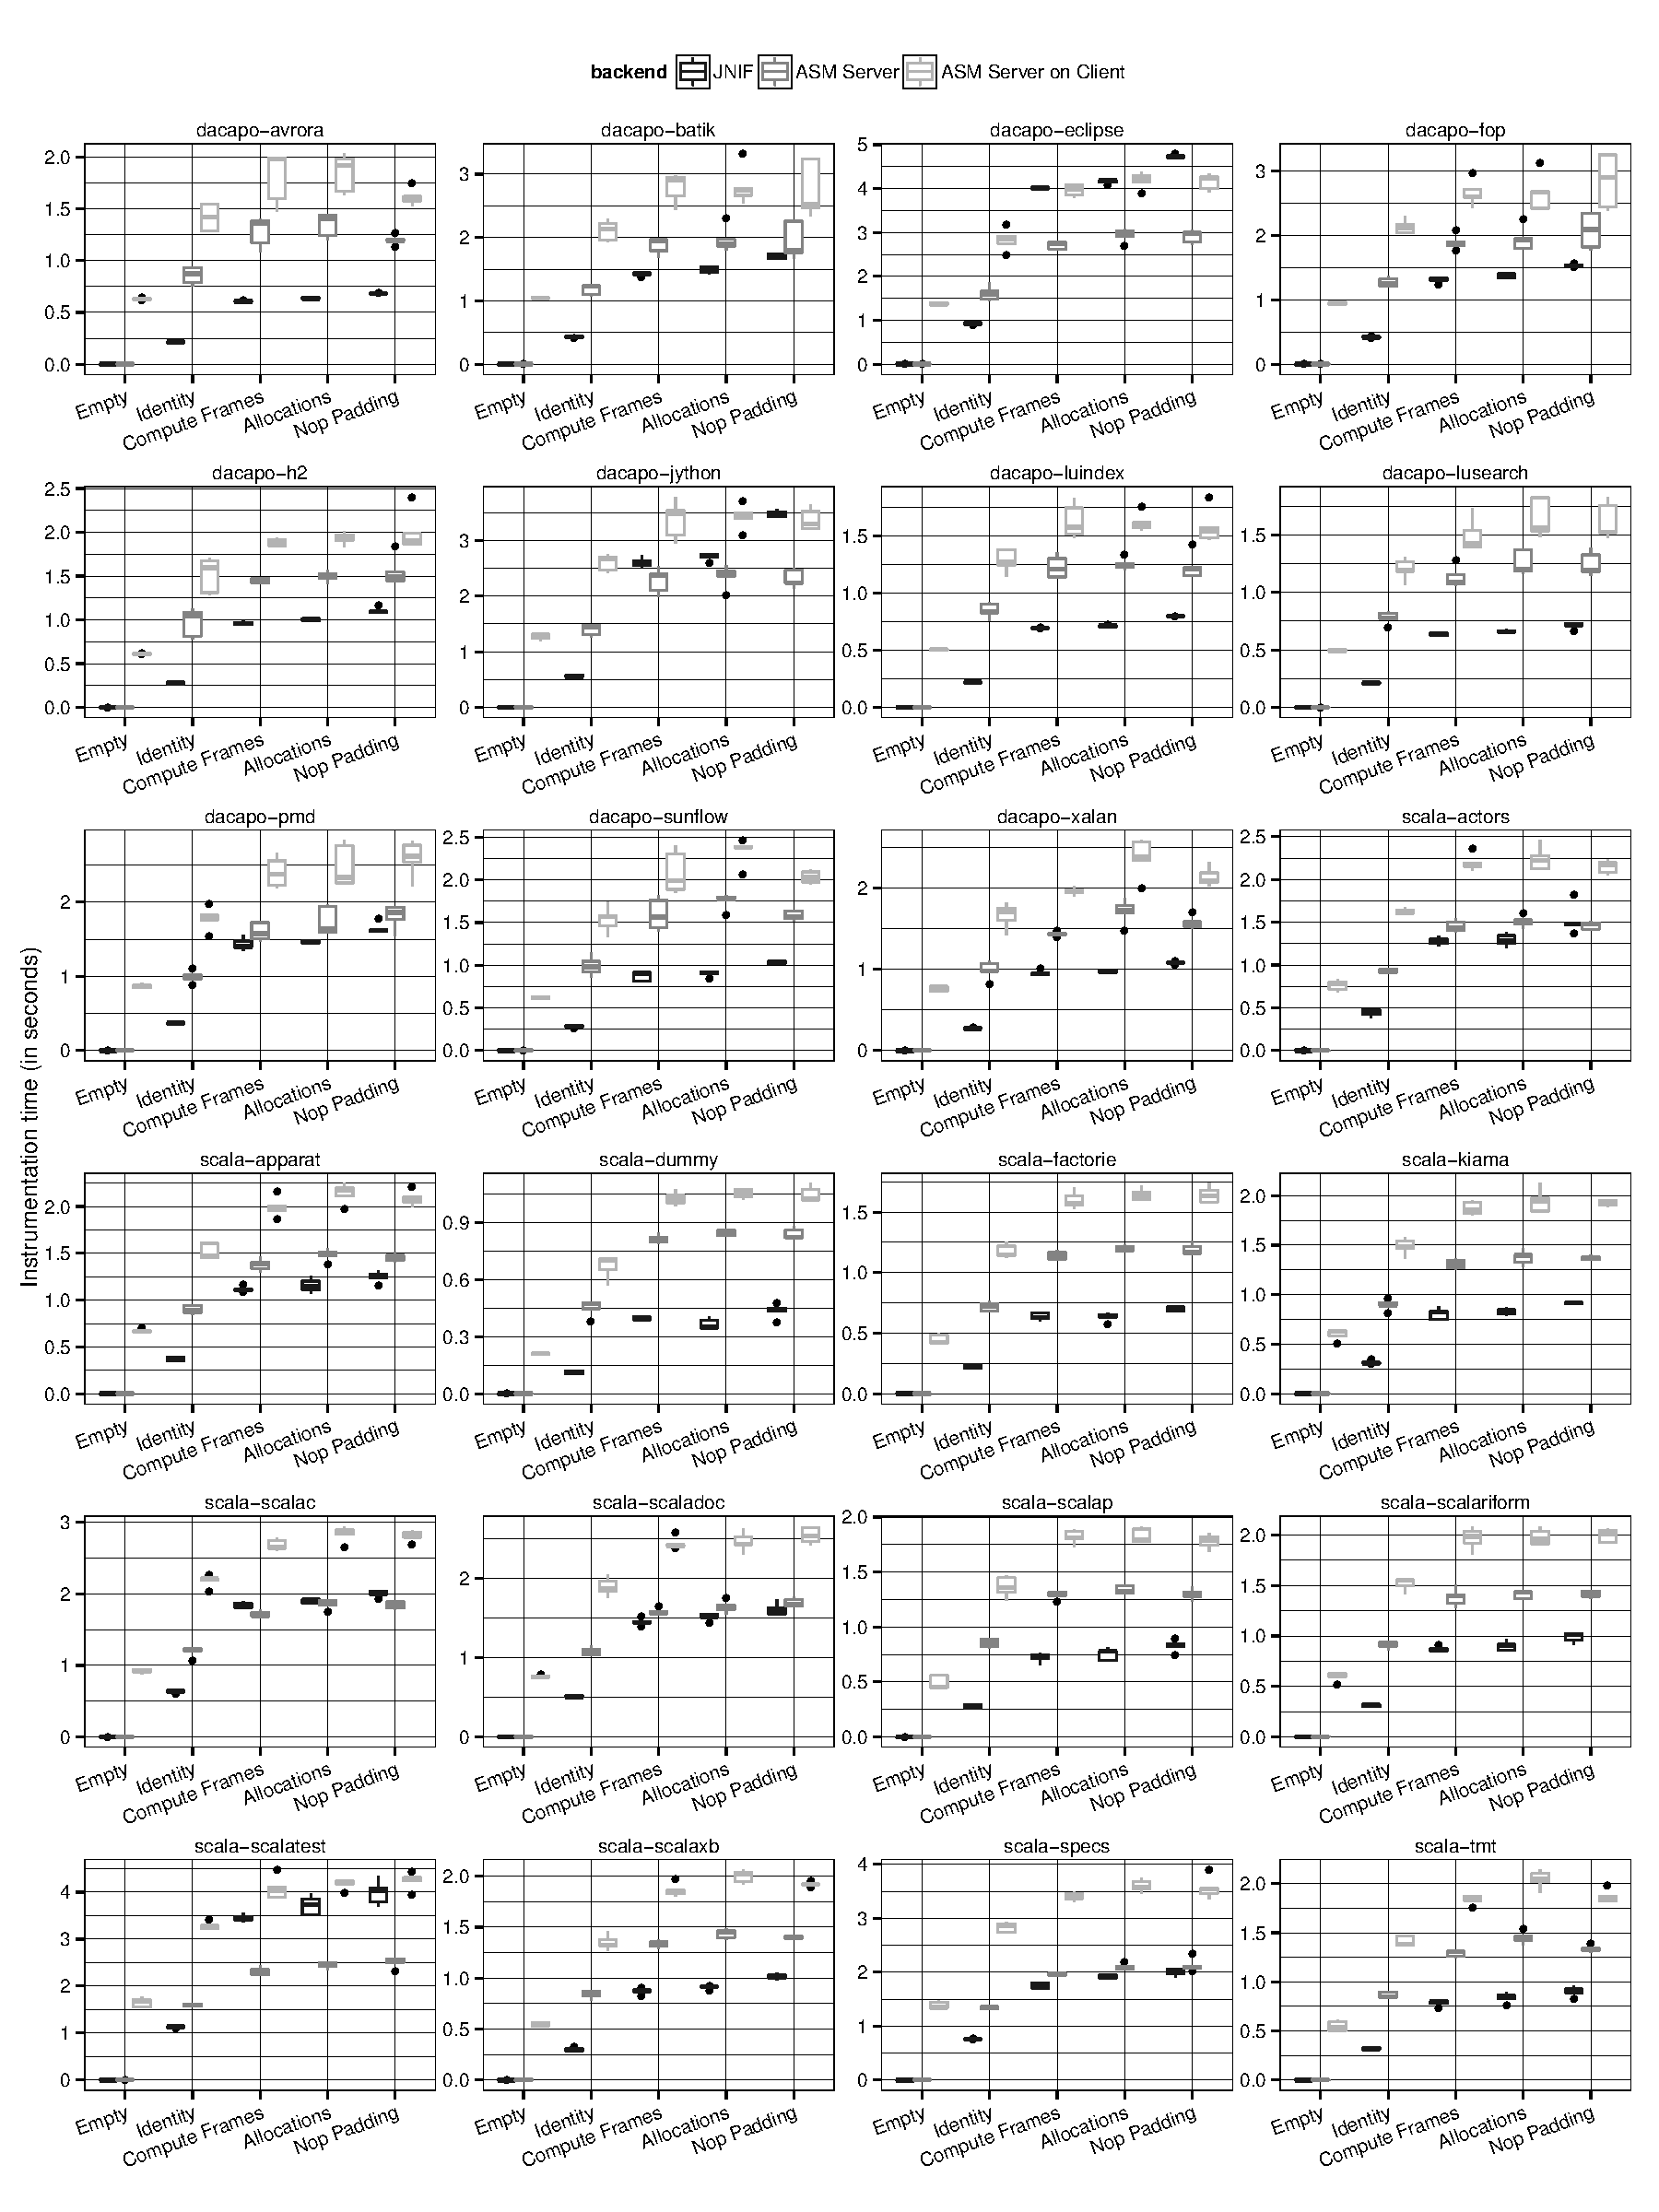
\includegraphics[width=\textwidth]{chapters/jnif/eval-all-chart-instr}

\vspace{-5mm}
\caption{Instrumentation time on DaCapo and Scala benchmarks}
\label{fig:instr-time}
\end{figure*}

%\chart{eval-dacapo-chart-instr}{Instrumentation time on DaCapo}{fig:instr-time-dacapo}
%\chart{eval-scala-chart-instr}{Instrumentation time on Scala and JRuby}{fig:instr-time-scala}

\subsection*{Reproducibility}

To run these evaluations, a Makefile script is provided in the git repository.
These tasks take care of the compilation of the JNIF library and also all java files needed. 
The repository is self-contained, no need to download dacapo benchmarks separately.

\begin{listing}
\begin{minted}[linenos=false]{text}
> make testapp
\end{minted}
\caption{Running testapp}
\label{usage-parse2}
\end{listing}

\begin{listing}
\begin{minted}[linenos=false]{text}
> make testapp
\end{minted}
\caption{Running dacapo}
\label{usage-parse3}
\end{listing}

To run a particular dacapo benchmark with default settings

\begin{listing}
\begin{minted}[linenos=false]{text}
> make dacapo BENCH=avrora
\end{minted}
\caption{Running dacapo}
\label{usage-parse4}
\end{listing}

To run a full evaluation with all dacapo benchmarks in all configuration a task -eval- is provided. You can set how many times run each configuration with the variable times, like

\begin{listing}
\begin{minted}[linenos=false]{text}
> make eval times=5
\end{minted}
\caption{Running full eval five times}
\label{usage-parse5}
\end{listing}

Finally, there is a task to create plots for the evaluation.
This task needs R with the package ggplot2.

\begin{listing}
\begin{minted}[linenos=false]{text}
> make plots
\end{minted}
\caption{Plots}
\label{usage-parse6}
\end{listing}

%1. Stand-alone test-unit:
%In this stage we only test basic functionality of the API such as get the
%right size and the ability to parse and write without correctly without
%any modification and with them. The use of this kind of tests rely on the
%property of the API that if no modification is done to the model the 
%writer is able to recover the original bytes of the class files (except with
%the non-unique property of the stack map tables).
%
%2. Minimal native agent:
%At this stage we prepared several kind of transformations (instrumentation)
%including the identity transformation to test if model/parser/analysis/writer
%can be executed correctly inside a JVM.
%
%3. Dacapo benchmarks:
%As the final tests we run those instrumentations on the Dacapo benchmarks 
%to stress the API. Moreover we use this stage to perform our evaluation.

\section{Limitations}
\label{sec:jnif-limitations}

JNIF still has some limitations.

\textbf{jsr/ret.} JNIF does not support stack map generation for jsr and ret.
Class files requiring stack maps do not include jsr/ret.
%Compute stack map frames for code with JSR/RET instructions not supported.
%JSR/RET makes the control flow graph generation difficult, because a RET instruction can jump to multiple targets instead of a predefined one.

\textbf{invokedynamic.} JNIF's support for invokedynamic is not yet fully tested, 
but our initial tests with JRuby have been successful
(using \texttt{-Djruby.compile.invokedynamic=true}).
% Since Dacapo bach was released in 2009 before the creation of Java 7 which introduces invokedynamic instruction, 
% it does not contain any benchmark with invokedynamic.
% Instead we use jruby 1.7 in order to create a self-contained jar file. 
% This jar file per does not contain any invokedynamic instruction, 
% but it does contain the jruby compiler, 
% that when specified via -Djruby.compile.invokedynamic=true it will generate class files with invokedynamic. 
% We tested our parser and writer with this settings with successful results.

\textbf{Stack map generation with full coverage.}
When the JVM loads the first few runtime library classes,
and calls the JVMTI agent to have those classes instrumented,
it is still too early to use JNI for loading classes needed for computing least upper bounds for stack map generation.
For this reason, we do not generate stack maps for runtime library classes.
This no problem, because the JVM does not verify the runtime library classes by default,
and thus it does not need stack maps for those classes.
However, should developers decide to explicitly turn on the verification of runtime library classes
(with \verb|-Xverify:all|), the verifier would complain because JNIF would not have generated stack maps.


% \ignore{
To get full coverage for the instrumentation inside a JVMTI agent, 
it is necessary to instrument every class, 
even the whole java class library.
If the instrumentation needs to change or add branch targets, 
the compute frames option must be used, 
but it cannot be used against the class library,
because to compute frames, 
the class hierarchy must be known, and 
this imposes a depedency with a classloader which is not yet available.

Luckily, by default the Java library classes are not verified, because they are trusted. 
Thus the instrumentation only needs to compute frames on classes not belonging to java library.

%Should developers wish to verify Java library classes anyways, they can use the \verb|-Xverify:all| option of the JVM.
% }
\section{Conclusions}
\label{sec:jnif-conclusions}

Until now, full-coverage dynamic instrumentation in production JVMs required performing the code rewriting in a separate JVM, 
because of the lack of a native bytecode rewriting framework.
This paper introduces JNIF, the first full-coverage in-process dynamic instrumentation framework for Java.
It discusses the key issues of creating such a framework for Java---such as stack-map generation---and
it evaluates the performance of JNIF against the most prevalent Java-level framework: ASM.
We find that JNIF is faster than using out-of-process ASM in most cases.
We hope that thanks to JNIF, and this paper, a broader number of researchers and developers will
be enabled to develop native JVM agents that analyze and rewrite Java bytecode without limitations. 


\chapter{Gathering Statistics using \ql{}}
\label{cha:ap:qlstats}

\begin{lstlisting}[style=ql]
//#lang=java
//#projectKeys=[25620005,41710041,1878521151,10560012,28580018,5629499534213120,39700035,1977701350,1873830050,1862920424,1864641207,1877441651,48190073,1506524326358,1505958786078,1506178136997,1981031959,1879370025,1874822090,1790840019,1864280925,41633751,1876381512,12760012,41900048,1354020033,1505967666111,1867300198,1795210073,1505968065973,1862771155,940125,2033800529,11020029,1505958645990,7870148,1861351166,1977291520,1978970761,1983122555,2161760237,1859762138,2035290917,1883290288,6890001,1981271240,1864352334,1979491471,1860005,13140029,24100035,35820136,1875601332,48640041,1877370912,1869242377,1872920090,1859802304,1973732641,1867040683,7880116,1971931877,33010046,18080071,1920002,1882261774,1855931308,1882380719,48790008,1505950676906,4870147,1860497242,1860885457,1883110029,1863051015,49820009,122244312,1861232120,1869270619,4850066,1872820788,6780442,1506173707109,1506179906986,32470022,1874830030,1797540044,1971780069,1968931653,1856951538,1908860284,1861491397,1884210730,1867130795,15070006,1798270110,46050017,1983122556,1856772013,35820134,1866091663,7860138,1866211423,1506494716249,1860946741,1505959776000,1880610249,1854901091,28741840,1972891707,6810158,1866061568,1982361113,1883200014,1505956416964,33815278,1869251537,1863190961,1874861017,1880570060,1863170850,1876500483,1873950073,1978970753,1878460091,1863001776,1874820078,7870357,10190041,1877480006,27300077,37220006,1882220728,1860774854,1977502912,1796321258,1877840310,2032670435,10130004,1971742352,1867160838,2980123,1878170062,1506502526259,1987320554,1862301883,1854881430,4840137,16030025,1505967225983,1855701520,1864150769,1859473908,1505958176673,2980106,1505964916170,1863840499,42360304,1984120998,1791770031,1506178546734,1856921186,1856830886,23842748,1506177197587,1857631417,1985420889,12170495,1861920745,1878800409,1860885493,1863511591,1876470319,3980080,17445104,5990306,1791430060,1344240419,1863420972,7870349,7890422,30640057,22650009,930029,1978821253,1868250766,1797370124,1973531692,7850125,1883460971,1984082076,1874820076,1874870633,20820034,30360001]

import java
import lang

predicate stats(string stat, int value) {
    ( stat = "CU" and value = count(CompilationUnit cu | cu.fromSource() ) ) or
    ( stat = "LOC" and value = sum(CompilationUnit cu || cu.getNumberOfLinesOfCode()) ) or
    ( stat = "Method" and value = count(Method m | exists(Block b | m.getBody() = b)) ) or
    ( stat = "MethodWithCast" and value = count(Callable m | exists(TypeCastExpr ce | ce.getEnclosingCallable() = m)) ) or
    ( stat = "Stmt" and value = count(Stmt s) ) or
    ( stat = "Expr" and value = count(Expr e) )
}

from string stat, int value
where stats(stat, value)
select stat, value
\end{lstlisting}

\backmatter

% \chapter{Glossary} %optional

%\bibliographystyle{alpha}
%\bibliographystyle{dcu}
\bibliographystyle{plainnat}
\bibliography{pubs}

% \cleardoublepage
% \theindex %optional, use only if you have an index, must use
	  %\makeindex in the preamble

\end{document}